%%%
%%% Main file of the thesis
%%%


\documentclass[a4paper,11pt,openany]{book} %Remove draft option to hide ToDos

%%%
%%% Shared preamble for all files, e.g. thesis, TikZ standalones, slides, etc.
%%% It defines \macros for types, Turing machines, etc.
%%%

% Packages needed
\usepackage[utf8]{inputenc}
\usepackage{geometry}
\usepackage[small,compact]{titlesec}
\usepackage[final]{listings}
\usepackage{amsmath}
\usepackage[amsmath,hyperref,thmmarks]{ntheorem}
% Warning: The package ntheorem defines a \None macro!
\usepackage{amssymb}
\usepackage{tipa}
\usepackage[english]{babel}
\usepackage{lstautogobble}
\usepackage{proof}
\usepackage{bussproofs}
\usepackage{xparse}
\usepackage{needspace}
\usepackage{xspace}
\usepackage{mathpartir}
\usepackage{stmaryrd} % for |llbracket and \rrbracket
\usepackage{standalone} % useful to out-source graphics


% TikZ ist *kein* Zeichenprogramm.
\usepackage{tikz}
\usetikzlibrary{arrows,shapes,snakes,automata,backgrounds,fit,positioning}
\usepackage{tikz-cd} % for commutative diagrams


%% Formating
\newcommand{\MS}[1]{\ensuremath{\mathsf{#1}}}
\newcommand{\MST}[1]{${\mathsf{#1}}$}
\newcommand{\IsMathMode}{\ifmmode{This is math mode}\else{This is not math mode}\fi}

%% Logic symbols
\newcommand{\defop}{\mathop{:=}}
\newcommand{\imp}{\mathbin{\rightarrow}~}
\newcommand{\Imp}{\mathbin{\Rightarrow}~}
\renewcommand{\iff}{\mathbin{\leftrightarrow}}


% ++ operator:
% Source: https://tex.stackexchange.com/questions/4194/how-to-typeset-haskell-operator-and-friends
\newcommand\doubleplus{+\kern-1.3ex+\kern0.8ex}
\newcommand\mdoubleplus{\ensuremath{\mathbin{+\mkern-10mu+}}}
\newcommand{\app}{\mdoubleplus}

\newcommand{\rew}{\Rightarrow}
\newcommand{\trew}{\stackrel{\textrm{T}}\Rightarrow}
\newcommand{\llrew}{\stackrel{\textrm{L}}\Rightarrow}
\newcommand{\rlrew}{\stackrel{\textrm{R}}\Rightarrow}
\newcommand{\arew}{\triangleright}
\newcommand{\conc}{\mathop{{+}\hskip-5pt{+}}}
\newcommand{\gen}{\Rightarrow}

%% Sets
% \newcommand{\lam}[2]{\lambda#1{.}\hskip.7pt#2}
\newcommand{\setOf}[1]{\bigl\{ #1 \bigr \}}
\newcommand{\setMap}[2]{\setOf{#1~\big|~#2}}
\newcommand{\depPair}[2]{\setOf{#1~{\&}~#2}}
\newcommand{\pair}[2]{\bigl( #1 , #2 \bigr)}
\newcommand{\class}[1]{\bigl[ #1 \bigr]}
\newcommand{\choice}[1]{\bigl< #1 \bigr>}
\newcommand{\explainRel}[2]{\stackrel{\text{#1}}{#2}}
\newcommand{\family}[2]{\bigl( #1 \bigr)_{#2}}
\newcommand{\from}{:}
\renewcommand{\to}{\rightarrow}

%% Types
\newcommand{\Bool}{\mathbb{B}}
\newcommand{\Fin}{\mathbb{F}}
\newcommand{\Nat}{\mathbb{N}}
\newcommand{\Prop}{\mathbb{P}}
\newcommand{\Type}{\mathbb{T}}
\newcommand{\Unit}{\MS{1}}
\newcommand{\Option}{\mathcal{O}}
\newcommand{\List}{\mathcal{L}}
\newcommand{\Rel}{\MS{Rel}}

\newcommand{\True}{\top}
\newcommand{\False}{\bot}

%% Tapes
\newcommand{\tape}[1]{[ #1 ]}
\newcommand{\tapePointer}[1]{\underset{\uparrow}{#1}}
\newcommand{\niltape}{\tape{\tapePointer{}}}
\newcommand{\midtape}[3]{\tape{#1~\tapePointer{#2}~#3}}
\newcommand{\leftof}[2]{\tape{\tapePointer{}~#1~#2}}
\newcommand{\rightof}[2]{\tape{#1~#2~\tapePointer{}}}

% \newcommand{\niltape}{\MS{niltape}}
% \newcommand{\midtape}[3]{\MS{midtape}~#1~#2~#3}
% \newcommand{\leftof}[2]{\MS{leftof}~#1~#2}
% \newcommand{\rightof}[2]{\MS{rightof}~#1~#2}

%% Turing machine types
\newcommand{\Loop}{\MS{loop}}
\newcommand{\Tape}{\MS{Tape}}
\newcommand{\Tapes}[1]{\Tape^{#1}}
\newcommand{\TM}{\MS{TM}}
\newcommand{\Move}{\MS{Move}}
\newcommand{\Act}{\MS{Act}}
\newcommand{\Conf}{\MS{Conf}}
\newcommand{\Tau}{\Gamma}

%% Relations
\newcommand{\rif}{\mathbin{\phi}}
\newcommand{\at} [2][]{#1{|}_{#2}}
\newcommand{\att}[2][]{#1{|\mkern-1.5mu|}_{#2}}
\DeclareMathOperator{\ignoreParam}{\Uparrow}
\DeclareMathOperator{\hideParam}{\Downarrow}


%% Constructors
\DeclareMathOperator{\inl}{\ensuremath{\MS{inl}}}
\DeclareMathOperator{\inr}{\ensuremath{\MS{inr}}}
\newcommand{\Some}[1]{\left\lfloor {#1} \right\rfloor}
% \None is defined sometimes
\renewcommand{\None}{\emptyset}
\newcommand{\true}{\MS{true}}
\newcommand{\false}{\MS{false}}
\newcommand{\unit}{\MS{()}}
\newcommand{\nil}{\MS{nil}}
\newcommand{\cons}{\mathbin{::}}

%% Functions
\newcommand{\map}[2]{\ensuremath{\MS{map}~#1~#2}}
\newcommand{\maptwo}[3]{\ensuremath{\MS{map}_2~#1~#2~#3}}
\newcommand{\rev}[1]{\MS{rev}~#1}

%% Vector
\newcommand{\Vector}[1]{\left[ #1 \right]}
\DeclareMathOperator{\hd}{\ensuremath{\MS{hd}}}
\DeclareMathOperator{\tl}{\ensuremath{\MS{tl}}}
\newcommand{\length}[1]{\left| #1 \right|}
\newcommand{\blength}[1]{\bigl| #1 \bigr|}


%%
%% Encding
%%
\newcommand{\contains}{\simeq}
\newcommand{\size}[1]{\length{encode(#1)}}

%% Semantics
\newcommand{\terminates}{\mathrel{\triangleright}}
\newcommand{\TerminatesIn}{\mathrel{\downarrow}}
\newcommand{\Realise}{\mathrel{\vDash}}
\newcommand{\RealiseIn}[1]{\mathrel{\vDash^{#1}}}

%%
%% Turing Machines
%%

%% Control flow operators
\newcommand{\While}{\MS{While}}
\newcommand{\Seq}{;~}
\newcommand{\Match}{\MS{Match}}
\newcommand{\If}[3]{\MS{If}~#1~\MS{Then}~#2~\MS{Else}~#3}
\newcommand{\Let}[2]{\MS{let}~#1~\MS{in}~#2}
\newcommand{\cond}[3]{\MS{if}~#1~\MS{then}~#2~\MS{else}~#3}
\newcommand{\Nop}{\MS{Nop}}
\newcommand{\Return}[2]{\MS{Return}~#1~#2}
% \newcommand{\Return}[2]{\MS{Return}_{#2}~#1}

%% Lifts
% #1 is the machine, #2 the lifting
\newcommand{\LiftTapes}[2]{\mathop{\Uparrow_{#2}} #1}
\newcommand{\LiftAlphabet}[2]{\mathop{\Uparrow_{#2}} #1}
% #1 is the machine, #2 the alphabet lifting, and #3 the tape-lifting
\newcommand{\LiftBoth}[3]{\mathop{\Uparrow_{#2;~#3}} #1}




%%%
%%% lstlisting
%%%

% Style and language to define complex multi-line definitions similar to Coq code
\lstdefinelanguage{semicoq}{
  keywords={if,then,else,true,false,match,Match,If,Then,Else,Nop,Return,Move,Reset,DoAct,WriteMove,L,R,N},
  comment=[s]{(*}{*)},
}

\lstdefinestyle{semicoqstyle}{
  mathescape=true,
  keywordstyle=\textsf,
  language=semicoq,
  literate={
    {=>}{{$\Rightarrow$}}2
    {>->}{{$\rightarrowtail\,$}}2
    {<->}{{$\leftrightarrow$ }}2
    {->}{{$\to$ }}3
    {~}{{$\lnot$}}1
    {/\\}{{$\land$}}2
    {\\/}{{$\lor$}}2
    {forall}{{$\forall$}}1
    {exists}{{$\exists$}}1
    {<>}{{$\not =$}}{1}
    {<=}{{$\leq$}}{1}
    {<}{{$\lt$}}{1}
    {>=}{{$\ge$}}{1}
    {>}{{$\gt$}}{1}
    % {Match}{$\mathsf{Match}$}{5}
    % {match}{$\textsf{match}$}{5}
    % {If}{$\MS{If}$}{5}
    % {if}{$\MS{if}$}{5}
    % {Then}{$\MS{Then}$}{5}
    % {then}{$\MS{then}$}{5}
    % {Else}{$\MS{Else}$}{5}
    % {else}{$\MS{else}$}{5}
  }
}

\lstdefinelanguage{pseudocode}{
  keywords={If,Then,Else,Do,While,Reset,Return},
}

\lstdefinestyle{pseudocode}{
  mathescape=true,
  language=pseudocode,
  literate={
    {:=}{{$\leftarrow$}}{1}
    {<>}{{$\not =$}}{1}
    {<=}{{$\leq$}}{1}
    {<}{{$\lt$}}{1}
    {>=}{{$\ge$}}{1}
    {>}{{$\gt$}}{1}
  }
}






%%% Local Variables:
%%% mode: LaTeX
%%% TeX-master: "thesis"
%%% End:
\include{header}
\tolerance=200

\settitle{Verified Programming of\\Turing Machines in Coq}
\setauthor{Maxi Wuttke}
\advisor{Yannick Forster}
\supervisor{Prof.\ Dr.\ Gert Smolka}
\reviewerOne{Prof.\ Dr.\ Gert Smolka}
\reviewerTwo{Prof.\ Dr.\ Holger Hermanns}
\university{Saarland University}
\faculty{Faculty of Mathematics and Computer Science}
\thesistype{Bachelor's}
\subdate{01}{September}{2018}
\city{Saarbr\"ucken}
\setBaseUrl{{https://www.ps.uni-saarland.de/~wuttke/bachelor/coqdoc/}}
\newcommand{\homepage}{https://www.ps.uni-saarland.de/~wuttke/bachelor/}

\DeclareTextFontCommand{\emph}{\bfseries}


\pagenumbering{roman}

\setlength{\headheight}{15pt}

\renewcommand{\chaptermark}[1]{ \markboth{#1}{} }
%\renewcommand{\sectionmark}[1]{ \markright{#1}{} }

\fancyhf{}
\fancyhead[LE,RO]{\thepage}
\fancyhead[RE]{\textit{ \nouppercase{\leftmark}} }
\fancyhead[LO]{\textit{ \nouppercase{\rightmark}} }

\fancypagestyle{plain}{
	\fancyhf{}
	\renewcommand{\headrulewidth}{0pt}
	\renewcommand{\footrulewidth}{0pt}
}

\makeglossaries

\begin{document}

\renewcommand\cite{\citep}

\pagestyle{empty}
\maketitlepage

% Empty page
\shipout\null

\statementpage

% Empty page
\shipout\null

\chapter*{Abstract}
%\addcontentsline{toc}{chapter}{\numberline{}Abstract}
Turing machines build the traditional foundation of the theory of computation and complexity.  However, concrete Turing machines are often only
sketched out.  Even if authors define the complete Turing machine, they leave the invariants to figure out for the reader.  Moreover, it is common to
employ the \textit{Church-Turing thesis}, to (informally) conclude that a function is Turing-computable.  Reasons for that are manifold.  Turing
machines are very low-level, because the operations on tapes are primitive.  They are also non-compositional; control-flow operators like sequential
composition and loops are not available.  Reasoning about invariants and concrete machine states is tedious, because the execution of the machine
could proceed from one state of the machine to any other state; the set of states may also be huge for complex machines.

In this thesis, we fill these gaps.  We present a framework developed in the theorem prover Coq, in that we can define, specify, and formally verify
multi-tape Turing machines.  The framework eases programming and verification of Turing machines, because it provides abstractions like values and
control-flow operators.  We showcase the power of this framework by programming and verifying a multi-tape Turing machine that simulates a two-stack
machine for the call-by-value $\lambda$-calculus.


%%% Local Variables:
%%% mode: LaTeX
%%% TeX-master: "thesis"
%%% End:

\newpage
% Empty page
\shipout\null

\chapter*{Acknowledgements}
I feel obliged to say special words of thank to Yannick Forster, who advised this thesis and the development of the framework presented in this
thesis.  In many weekly meetings, over the course of one year, we discussed how the framework could look like.  Over the course of the development, he
also helped me to organise myself.  I am thankful that he provided a {\LaTeX} template for this thesis and that he proof read my texts many times.

I want to thank my supervisor Prof.~Smolka, who introduced me to the field of functional programming and computational logic.  I always appreciated
his passion in his lectures.  Without him, I would not have found the field of computational logic and formal verification.  I also recognise the help
of Kathrin Stark, who helped me getting into this topic, in particular because I missed the first three weeks of \textit{Introduction to Computational
  Logic}.  I want to thank Prof.~Smolka for giving me the opportunity to write my thesis at his chair.  I really appreciate the atmosphere together
with motivated PhD students, especially with Kathrin Stark, Fabian Kunze, and Yannick Forster.

I express gratitude to Prof.~Hermanns, who mentored me in the computer science undergraduate Honours Program of Saarland University.  I am glad that
he is the second reviewer of this thesis.

Lastly, I want to thank my parents for supporting me in every imaginable way.  Without my parents, this thesis would not exists, me neither.


%%% Local Variables:
%%% TeX-master: "thesis"
%%% mode: LaTeX
%%% End:


\newpage
% Empty page
\shipout\null

\tableofcontents

\listoftodos

\clearpage
\pagestyle{fancy}
\pagenumbering{arabic}

% Include all chapters here
\chapter{Introduction}
\label{chap:intro}


Turing machines are the foundation of complexity theory.  However, reasoning about Turing machines 


\section{Related Work}
\label{sec:relatedwork}

\todo{``et~al.'' or ``et~al''?}

Asperti and Ricciotti \cite{asperti2012} formalise single-tape Turing machines over arbitrary alphabets in the proof assistant \textit{Matita}.  They
also \cite{asperti2015} formalise multi-tape Turing machines in Matita.  They use the notion of \textit{realisation} of relations for specifying
semantics of Turing machines.

Xu, Zhang, and Urban \cite{Xu:2013:MTM:2529315.2529331} formalise single-tape Turing machines over a binary alphabet in Isabelle/HOL.  They follow the
textbook of Boolos et~al~\cite{boolos2007computability} and use Hoare-logic to specify the semantics of Turing machines.  They translate
\textit{abacus programs} to Turing machines and prove the undecidable of the halting problem of Turing machines.

Ciaffaglione et~al~\cite{Ciaffaglione:2016:TTC:2956213.2956306} define tapes of Turing machines as infinite streams.  They certify Turing machines
using induction and co-induction in Coq.

\todo{she? How to properly cite bachelor's theses?}
In her bachelor thesis, Heiter~\cite{Heiter} reduces the halting problem of single-tape to the \textit{Post correspondence problem} in Coq.  She uses
the same definition of single-tape Turing machines as in \cite{asperti2012}.


\section{Contributions}
\label{sec:contributions}

\section{Outline}
\label{sec:outline}

In Chapter \ref{chap:definitions}, the notion of multi-tape Turing machines is defined.  We also introduce means to specify the semantics of machines,
and define some basic machines.

Chapter \ref{chap:combining} defines control-flow operators and shows how we can combine machines.  We also show how to build some not-so-complex
machine.

In Chapter \ref{chap:programming}, we introduce abstractions, like value-containing and computation of functions.  We introduce a general pattern, how
to program multi-tape Turing machines; this pattern is followed in some case-studies.

In Chapter \ref{chap:heap}, we use all technics developed in this thesis, to build a machine that simulates an abstract heap machine.  From the
correctness of this Turing machine, we conclude that the halting problem of the abstract machine reduces to the halting problem of multi-tape Turing
machines.

We discuss some technical difficulties of our Coq-implementation in Chapter \ref{chap:implementation}.

Chapter \ref{chap:conclusion} concludes, and lists possibilities for future work.

\todo{Continuity, hierarchy}


%%% Local Variables:
%%% TeX-master: "thesis"
%%% End:

\chapter{Definitions}
\label{chap:definitions}

In this chapter, we will formally define the notion of multi-tape Turing machines.
(Our definitions are based on Asperti et al.)

We will introduce our notions for specifying the semantics of machines.

We will define some basic machines, state and proof their correctness, using the definitions and lemmas developed in this chapter.

\section{Machines and Tapes}
\label{sec:machine_tapes}

\section{Specification of Semantic}
\label{sec:spec_semantics}

\section{Basic Machines}
\label{sec:basic_machines}

%%% Local Variables:
%%% TeX-master: "thesis"
%%% End:

\chapter{Primitive Machines}
\label{chap:basic}

In this chapter, we define several classes of \textit{primitive} machines.\footnote{Asperti and Ricciotti~\cite{asperti2015} call these machines
  \textit{basic} machines.}  These machines are defined on an arbitrary finite alphabet $\Sigma$, but they have at most one tape, and they terminate
after at most one transition.  Primitive machines are the only concrete machines for that we give transition functions $\delta$ explicitly.  They are
also the only concrete machines, for that we fully specify the type of machine states $Q$.  In the following two chapters, we will show how to combine
these machines and build (and verify) complex machines without mentioning $Q$ or $\delta$ again.  All states and transition functions will be derived
from these machines.


\section{$\MS{Null}$}
\label{sec:Null}

\setCoqFilename{ProgrammingTuringMachines.TM.Basic.Null}


The machine $\MS{Null}_\Sigma$ is parametrised over the alphabet $\Sigma$.  Because $\Sigma$ is always clear from the context, we leave the index out.
We fix an alphabet $\Sigma$.  $\MS{Null}$ has zero tapes and terminates immediately, i.e.\ after $0$ steps.

\begin{definition}[$\MS{Null}$][Null]
  \label{def:Null}
  $\MS{Null} : \TM_\Sigma^{\mkern+1mu 0}$ is defined as follows:
  \begin{align*}
    Q          &:= \Unit \\
    start      &:= \unit \\
    \delta ~\_ &:= (\unit, \nil) \\
    halt   ~\_ &:= \true
  \end{align*}
\end{definition}
Note that if we have an unlabelled machine $M:\TM_\Sigma^n$, we implicitly label their states over $\Unit$ with the labelling function
$lab_M(q):=\unit$.

% The correctness relation says exactly that the tapes don't change:
The correctness relation is the universal relation, because empty vectors do not have information.  However, the correctness lemma also states that
the machine terminates in $0$ steps.
\begin{lemma}[Correctness of $\MS{Null}$][Null_Sem]
  \label{lem:Null_Sem} $\MS{Null} \RealiseIn0 NullRel$ with $NullRel := \lambda~t~t'.~ \True$.
\end{lemma}
\begin{proof}
  By execution.  The machine terminates after zero steps in the state $\unit$.
\end{proof}

\section{$\MS{DoAct}$}
\label{sec:DoAct}

\setCoqFilename{ProgrammingTuringMachines.TM.Basic.Mono}

Machines of the next class, $\MS{DoAct}~a : \TM_\Sigma^1(L)$, do only one action $a:\Act$ (i.e.\ they optionally write a symbol and move the head of
the tape) and terminate.
\begin{definition}[$\MS{DoAct}~a$][DoAct]
  \label{def:DoAct}
  Let $a:\Act_\Sigma$.  Then $\MS{DoAct}~a : \TM_\Sigma^1$ is defined as follows:
  \begin{align*}
    Q          &:= \Bool \\
    start      &:= \false \\
    \delta ~\_ &:= (\true, \Vector{a}) \\
    halt   ~ b &:= b
  \end{align*}
\end{definition}
The semantics of $\MS{DoAct}$ is easily expressed using the function $\MS{doAct}$ (see Definition~\ref{def:step}).  The machine terminates after one
transition:
\begin{lemma}[Correctness of $\MS{DoAct}$][DoAct_Sem]
  \label{lem:DoAct_Sem} $\MS{DoAct}~a \RealiseIn1 DoActRel~a$ with
  \[
    DoActRel~a := \lambda t~t'.~ t'[0] = \MS{doAct}~t[0]~a.
  \]
\end{lemma}
% \begin{proof}
%   By execution.
% \end{proof}
We define some abbreviations:
\begin{definition}[Machine classes derived from $\MS{DoAct}$][DoAct_Derived]
 \label{def:DoAct-derived} 
 \begin{align*}
   \MS{Move}       ~d &:= \MS{DoAct} (\None, d) \\
   \MS{Write}    ~s   &:= \MS{DoAct} (\Some{s}, \MS{N}) \\
   \MS{WriteMove}~s~d &:= \MS{DoAct} (\Some{s}, d)
 \end{align*}
\end{definition}


\section{$\MS{Read}$}
\label{sec:basic_machines-Read}

$\MS{Read} : \TM_\Sigma^1(\Option(\Sigma))$ is an interesting class of labelled one-tape machines.  The machines of this class have one terminating
state for each symbol of the alphabet $\Sigma$.  They read the current symbol from the tape and terminate in the state that corresponds to that
symbol.  For the case that there is no current symbol, they also have a distinct terminating state.  The labelling function maps the terminating state
for the symbol $s$ to the label $\Some{s}$.

\begin{definition}[$\MS{Read}$][ReadChar]
  The machine $\MS{Read} : \TM_\Sigma^1(\Option(\Sigma))$ is defined as follows:
  \begin{align*}
    Q          &:= \Bool+\Sigma \\
    start      &:= \inl \false \\
    \delta (\_, s) &:=
                     \begin{cases}
                       (\inl \true, \Vector{(\None, N)}) & s[0] = \None \\
                       (\inr c, \Vector{(\None, N)})     & s[0] = \Some c
                     \end{cases} \\
    halt   ~ (\inl  b) &:= b \\
    halt   ~ (\inr \_) &:= \true \\
    lab    ~ (\inl \_) &:= \None \\
    lab    ~ (\inr  s) &:= \Some s
  \end{align*}
\end{definition}

The correctness lemma of $\MS{Read}$ states that the machine terminates after one step, leaves the tape unchanged, and that the label of the
terminating state corresponds to the current symbol on the tape.

\begin{lemma}[Correctness of $\MS{Read}$][ReadChar_Sem]
  \label{lem:Read_Sem} $\MS{Read} \RealiseIn{1} ReadRel$ with
  \[
    ReadRel := \lambda~t~(l,t').~ l = \MS{current}~t[0] \land t' = t
  \]
\end{lemma}
\begin{proof}
  Case distinction over $\MS{current}~t[0]$.  Both cases follow by executing the machine one step.
\end{proof}


%%% Local Variables:
%%% TeX-master: "thesis"
%%% End:
\chapter{Combining Turing Machines}
\label{chap:combining}

In Chapter \ref{chap:definitions}, we have defined the notion of multi-tape Turing machines and basic machines.  In this chapter, we want to construct
more complex machines, for example a single-tape machine that moves the head to the right or to a certain symbol.
We define control flow operators, like ``match'', ``if then else'', ``sequential composition'', and ``while''.
As a result, we get a shallow-embed-ed language for programming multi-tape Turing machines in an imperative way.

\section{Match}
\label{sec:match}

Asperti and Ricciotti~\cite{asperti2015} also define the control flow operators sequential composition, conditional, and while.  However, for the
conditional they have to give one explicit ``else'' state.  Giving an explicit state is very tedious for complex machines.  That is why we use the
generalised notion of partitioned machines.  For example, for the conditional $\If{M_1}{M_2}{M_3}$, $M_1$ is partitioned over $\Bool$.  If $M_1$
terminated in a ``positive'' state (i.e. a state belonging to the partition $\true$), $M_2$ is executed after $M_1$.  Else it executes $M_3$ after
$M_1$.  We observe that sequential composition and conditional can be defined as instances of a more general operator we call $\MS{Match}$.  We give
proof scratches for the correctness and runtime in Subsection~\ref{sec:match-proofs}.

Let $M : \TM_\Sigma^n(F)$ and $M' \from F \to \TM_\Sigma^n(F')$ be a function from partitions to machines.  We define
$\MS{Match}~M~M' : \TM_\Sigma^n(F')$.

\begin{definition}[$\MS{Match}~M~M'$]
  \label{def:Match}
  \begin{alignat*}{3}
    & Q                  &~:=~& Q_M +  \sum_{y:F} Q_{M'(y)} \\
    & start              &~:=~& \inl start_M \\
    \delta ~&(\inl q, s) &~:=~&
    \begin{cases}
      \bigl(\inr (part_M~q, start_{M' (part_M~q)}), (\None, N)^n \bigr) & halt_M(q) \\
      \Let{(q', a) := \delta_M(q, s)}{\left(\inl q', a \right)} & \lnot halt_M(q)
    \end{cases} \\
    \delta ~&(\inr q, s) &~:=~& \Let{(q', a) := \delta_{M'(\pi_1 q)} (\pi_2 q, s)}{\bigl( \inr (\pi_1 q, q'), a \bigr)} \\
    halt   ~&(\inl  q)   &~:=~& \false \\
    halt   ~&(\inr  q)   &~:=~& halt_{M'(\pi_1~q)} (\pi_2~q) \\
    part   ~&(\inl  q)   &~:=~& \_ \\
    part   ~&(\inr  q)   &~:=~& part_{M'(\pi_1~q)} (\pi_2~q)
  \end{alignat*}
\end{definition}

In Definition~\ref{def:Match}, the $part$ value for $\inl$ is unimportant, because the states of $M_1$ are not terminating states.  We just use a
canonical value.

\begin{figure}
  \center
  \documentclass{standalone}

%%%
%%% Shared preamble for all files, e.g. thesis, TikZ standalones, slides, etc.
%%% It defines \macros for types, Turing machines, etc.
%%%

% Packages needed
\usepackage[utf8]{inputenc}
\usepackage{geometry}
\usepackage[small,compact]{titlesec}
\usepackage[final]{listings}
\usepackage{amsmath}
\usepackage[amsmath,hyperref,thmmarks]{ntheorem}
% Warning: The package ntheorem defines a \None macro!
\usepackage{amssymb}
\usepackage{tipa}
\usepackage[english]{babel}
\usepackage{lstautogobble}
\usepackage{proof}
\usepackage{bussproofs}
\usepackage{xparse}
\usepackage{needspace}
\usepackage{xspace}
\usepackage{mathpartir}
\usepackage{stmaryrd} % for |llbracket and \rrbracket
\usepackage{standalone} % useful to out-source graphics


% TikZ ist *kein* Zeichenprogramm.
\usepackage{tikz}
\usetikzlibrary{arrows,shapes,snakes,automata,backgrounds,fit,positioning}
\usepackage{tikz-cd} % for commutative diagrams


%% Formating
\newcommand{\MS}[1]{\ensuremath{\mathsf{#1}}}
\newcommand{\MST}[1]{${\mathsf{#1}}$}
\newcommand{\IsMathMode}{\ifmmode{This is math mode}\else{This is not math mode}\fi}

%% Logic symbols
\newcommand{\defop}{\mathop{:=}}
\newcommand{\imp}{\mathbin{\rightarrow}~}
\newcommand{\Imp}{\mathbin{\Rightarrow}~}
\renewcommand{\iff}{\mathbin{\leftrightarrow}}


% ++ operator:
% Source: https://tex.stackexchange.com/questions/4194/how-to-typeset-haskell-operator-and-friends
\newcommand\doubleplus{+\kern-1.3ex+\kern0.8ex}
\newcommand\mdoubleplus{\ensuremath{\mathbin{+\mkern-10mu+}}}
\newcommand{\app}{\mdoubleplus}

\newcommand{\rew}{\Rightarrow}
\newcommand{\trew}{\stackrel{\textrm{T}}\Rightarrow}
\newcommand{\llrew}{\stackrel{\textrm{L}}\Rightarrow}
\newcommand{\rlrew}{\stackrel{\textrm{R}}\Rightarrow}
\newcommand{\arew}{\triangleright}
\newcommand{\conc}{\mathop{{+}\hskip-5pt{+}}}
\newcommand{\gen}{\Rightarrow}

%% Sets
% \newcommand{\lam}[2]{\lambda#1{.}\hskip.7pt#2}
\newcommand{\setOf}[1]{\bigl\{ #1 \bigr \}}
\newcommand{\setMap}[2]{\setOf{#1~\big|~#2}}
\newcommand{\depPair}[2]{\setOf{#1~{\&}~#2}}
\newcommand{\pair}[2]{\bigl( #1 , #2 \bigr)}
\newcommand{\class}[1]{\bigl[ #1 \bigr]}
\newcommand{\choice}[1]{\bigl< #1 \bigr>}
\newcommand{\explainRel}[2]{\stackrel{\text{#1}}{#2}}
\newcommand{\family}[2]{\bigl( #1 \bigr)_{#2}}
\newcommand{\from}{:}
\renewcommand{\to}{\rightarrow}

%% Types
\newcommand{\Bool}{\mathbb{B}}
\newcommand{\Fin}{\mathbb{F}}
\newcommand{\Nat}{\mathbb{N}}
\newcommand{\Prop}{\mathbb{P}}
\newcommand{\Type}{\mathbb{T}}
\newcommand{\Unit}{\MS{1}}
\newcommand{\Option}{\mathcal{O}}
\newcommand{\List}{\mathcal{L}}
\newcommand{\Rel}{\MS{Rel}}

\newcommand{\True}{\top}
\newcommand{\False}{\bot}

%% Tapes
\newcommand{\tape}[1]{[ #1 ]}
\newcommand{\tapePointer}[1]{\underset{\uparrow}{#1}}
\newcommand{\niltape}{\tape{\tapePointer{}}}
\newcommand{\midtape}[3]{\tape{#1~\tapePointer{#2}~#3}}
\newcommand{\leftof}[2]{\tape{\tapePointer{}~#1~#2}}
\newcommand{\rightof}[2]{\tape{#1~#2~\tapePointer{}}}

% \newcommand{\niltape}{\MS{niltape}}
% \newcommand{\midtape}[3]{\MS{midtape}~#1~#2~#3}
% \newcommand{\leftof}[2]{\MS{leftof}~#1~#2}
% \newcommand{\rightof}[2]{\MS{rightof}~#1~#2}

%% Turing machine types
\newcommand{\Loop}{\MS{loop}}
\newcommand{\Tape}{\MS{Tape}}
\newcommand{\Tapes}[1]{\Tape^{#1}}
\newcommand{\TM}{\MS{TM}}
\newcommand{\Move}{\MS{Move}}
\newcommand{\Act}{\MS{Act}}
\newcommand{\Conf}{\MS{Conf}}
\newcommand{\Tau}{\Gamma}

%% Relations
\newcommand{\rif}{\mathbin{\phi}}
\newcommand{\at} [2][]{#1{|}_{#2}}
\newcommand{\att}[2][]{#1{|\mkern-1.5mu|}_{#2}}
\DeclareMathOperator{\ignoreParam}{\Uparrow}
\DeclareMathOperator{\hideParam}{\Downarrow}


%% Constructors
\DeclareMathOperator{\inl}{\ensuremath{\MS{inl}}}
\DeclareMathOperator{\inr}{\ensuremath{\MS{inr}}}
\newcommand{\Some}[1]{\left\lfloor {#1} \right\rfloor}
% \None is defined sometimes
\renewcommand{\None}{\emptyset}
\newcommand{\true}{\MS{true}}
\newcommand{\false}{\MS{false}}
\newcommand{\unit}{\MS{()}}
\newcommand{\nil}{\MS{nil}}
\newcommand{\cons}{\mathbin{::}}

%% Functions
\newcommand{\map}[2]{\ensuremath{\MS{map}~#1~#2}}
\newcommand{\maptwo}[3]{\ensuremath{\MS{map}_2~#1~#2~#3}}
\newcommand{\rev}[1]{\MS{rev}~#1}

%% Vector
\newcommand{\Vector}[1]{\left[ #1 \right]}
\DeclareMathOperator{\hd}{\ensuremath{\MS{hd}}}
\DeclareMathOperator{\tl}{\ensuremath{\MS{tl}}}
\newcommand{\length}[1]{\left| #1 \right|}
\newcommand{\blength}[1]{\bigl| #1 \bigr|}


%%
%% Encding
%%
\newcommand{\contains}{\simeq}
\newcommand{\size}[1]{\length{encode(#1)}}

%% Semantics
\newcommand{\terminates}{\mathrel{\triangleright}}
\newcommand{\TerminatesIn}{\mathrel{\downarrow}}
\newcommand{\Realise}{\mathrel{\vDash}}
\newcommand{\RealiseIn}[1]{\mathrel{\vDash^{#1}}}

%%
%% Turing Machines
%%

%% Control flow operators
\newcommand{\While}{\MS{While}}
\newcommand{\Seq}{;~}
\newcommand{\Match}{\MS{Match}}
\newcommand{\If}[3]{\MS{If}~#1~\MS{Then}~#2~\MS{Else}~#3}
\newcommand{\Let}[2]{\MS{let}~#1~\MS{in}~#2}
\newcommand{\cond}[3]{\MS{if}~#1~\MS{then}~#2~\MS{else}~#3}
\newcommand{\Nop}{\MS{Nop}}
\newcommand{\Return}[2]{\MS{Return}~#1~#2}
% \newcommand{\Return}[2]{\MS{Return}_{#2}~#1}

%% Lifts
% #1 is the machine, #2 the lifting
\newcommand{\LiftTapes}[2]{\mathop{\Uparrow_{#2}} #1}
\newcommand{\LiftAlphabet}[2]{\mathop{\Uparrow_{#2}} #1}
% #1 is the machine, #2 the alphabet lifting, and #3 the tape-lifting
\newcommand{\LiftBoth}[3]{\mathop{\Uparrow_{#2;~#3}} #1}




%%%
%%% lstlisting
%%%

% Style and language to define complex multi-line definitions similar to Coq code
\lstdefinelanguage{semicoq}{
  keywords={if,then,else,true,false,match,Match,If,Then,Else,Nop,Return,Move,Reset,DoAct,WriteMove,L,R,N},
  comment=[s]{(*}{*)},
}

\lstdefinestyle{semicoqstyle}{
  mathescape=true,
  keywordstyle=\textsf,
  language=semicoq,
  literate={
    {=>}{{$\Rightarrow$}}2
    {>->}{{$\rightarrowtail\,$}}2
    {<->}{{$\leftrightarrow$ }}2
    {->}{{$\to$ }}3
    {~}{{$\lnot$}}1
    {/\\}{{$\land$}}2
    {\\/}{{$\lor$}}2
    {forall}{{$\forall$}}1
    {exists}{{$\exists$}}1
    {<>}{{$\not =$}}{1}
    {<=}{{$\leq$}}{1}
    {<}{{$\lt$}}{1}
    {>=}{{$\ge$}}{1}
    {>}{{$\gt$}}{1}
    % {Match}{$\mathsf{Match}$}{5}
    % {match}{$\textsf{match}$}{5}
    % {If}{$\MS{If}$}{5}
    % {if}{$\MS{if}$}{5}
    % {Then}{$\MS{Then}$}{5}
    % {then}{$\MS{then}$}{5}
    % {Else}{$\MS{Else}$}{5}
    % {else}{$\MS{else}$}{5}
  }
}

\lstdefinelanguage{pseudocode}{
  keywords={If,Then,Else,Do,While,Reset,Return},
}

\lstdefinestyle{pseudocode}{
  mathescape=true,
  language=pseudocode,
  literate={
    {:=}{{$\leftarrow$}}{1}
    {<>}{{$\not =$}}{1}
    {<=}{{$\leq$}}{1}
    {<}{{$\lt$}}{1}
    {>=}{{$\ge$}}{1}
    {>}{{$\gt$}}{1}
  }
}






%%% Local Variables:
%%% mode: LaTeX
%%% TeX-master: "thesis"
%%% End:

\begin{document}
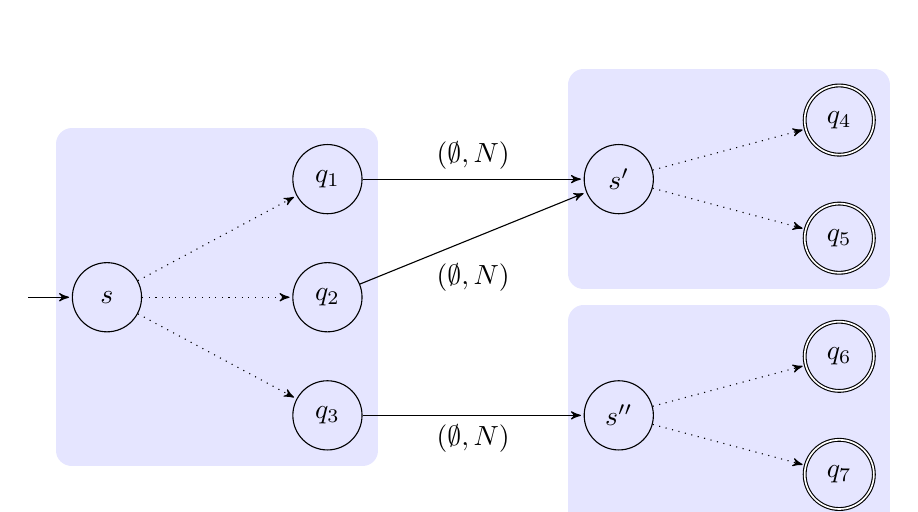
\begin{tikzpicture}[->,>=stealth',shorten >=1pt,auto,node distance=2.8cm]
  \begin{scope}
	  % Machine M
	  \node[state]          (M init)                                    {$s$};
	  \node[state]          (M exit 1)  [right of=M init,yshift= 1.5cm] {$q_1$};
	  \node[state]          (M exit 2)  [right of=M init,yshift= 0.0cm] {$q_2$};
	  \node[state]          (M exit 3)  [right of=M init,yshift=-1.5cm] {$q_3$};
	  \path (M init)
	  edge[dotted] (M exit 1)
	  edge[dotted] (M exit 2)
	  edge[dotted] (M exit 3);
	  \path (M init) ++(-1.0,0) edge (M init);
  \end{scope}
  \begin{scope}[xshift=6.5cm]
	  % Match-Machines
	  \begin{scope}[yshift=1.5cm]
		  % Accepting match machine
		  \node[state]          (M 1 init)                                        {$s'$};
		  \node[state, double]  (M 1 exit 1)  [right of=M 1 init, yshift= 0.75cm] {$q_4$};
		  \node[state, double]  (M 1 exit 2)  [right of=M 1 init, yshift=-0.75cm] {$q_5$};
		  \path (M 1 init)
		  edge[dotted] (M 1 exit 1)
		  edge[dotted] (M 1 exit 2);
	  \end{scope}
	  \begin{scope}[yshift=-1.5cm]
		  % Accepting match machine
		  \node[state]          (M 2 init)                                        {$s''$};
		  \node[state, double]  (M 2 exit 1)  [right of=M 2 init, yshift= 0.75cm] {$q_6$};
		  \node[state, double]  (M 2 exit 2)  [right of=M 2 init, yshift=-0.75cm] {$q_7$};
		  \path (M 2 init)
		  edge[dotted] (M 2 exit 1)
		  edge[dotted] (M 2 exit 2);
	  \end{scope}
  \end{scope}
  % Connecting edges
  \path
  (M exit 1) edge node[anchor=south] {$(\emptyset, N)$} (M 1 init)
  (M exit 2) edge node[anchor=north,yshift=-0.2cm] {$(\emptyset, N)$} (M 1 init)
  (M exit 3) edge node[anchor=north] {$(\emptyset, N)$} (M 2 init);

  \begin{pgfonlayer}{background}
	  \filldraw [line width=4mm,join=round,blue!10]
	  (M   exit 1.north -| M   init.west) rectangle (M   exit 3.south -| M   exit 3.east)
	  (M 1 exit 1.north -| M 1 init.west) rectangle (M 1 exit 2.south -| M 1 exit 2.east)
	  (M 2 exit 1.north -| M 2 init.west) rectangle (M 2 exit 2.south -| M 2 exit 2.east);
  \end{pgfonlayer}
\end{tikzpicture}

\end{document}


%%% Local Variables:
%%% TeX-master: t
%%% End:
  \caption{Example of a $\MS{Match}$.  The left box stands for the first machine $M_1:\TM_\Sigma^n(\Bool)$.  The states $q_1$ and $q_2$ are mapped to
    $\true$, $q_3$ is mapped to $\false$.  After the $\MS{Match}$ reaches one of the injections of the terminal states $q_1, \cdots, q_3$ of $M_1$, it
    continues its execution either in the top case machine $M_2$ or in the bottom case machine $M_3$.  The halting states of $\MS{Match}$ are exactly
    the injections of the halting states of the case-machines.}
  \label{fig:match}
\end{figure}

\todo{Maybe use parenthesises, e.g.\ $\Match(M,M')$ and $MS{MatchRel}(R,R')$ for better readability}


$\MS{Match}~M~M'$ first executes a copy of $M$.  When it reaches a final state $q$ of $M$, it does a ``nop'' action (i.e.\ $(\None,N)^n$) and changes
to to the injection of the start state of the machine $M'(part~q)$.  When $\MS{Match}~M~M'$ reaches a state that is the injection of a final state of
a machine $M'~y$, it terminates.  The correctness part of the semantics can be expressed using the following lemma:

\begin{lemma}[Correctness of $\MS{Match}~M~M'$]
  \label{lem:Match_Realise}
  Let $R \subseteq \Tape_\Sigma^n \times F \times \Tape_\Sigma^n$ and $R'~y \subseteq \Tape_\Sigma^n \times F' \times \Tape_\Sigma^n$ for all $y:F$.
  If $M \vDash R$ and $M'~y \vDash R'~y$ for all $y:F$, then
  \[
    \MS{Match}~M~M' \vDash \MS{MatchRel}~R~R'
  \]
  with
  \[
    \MS{MatchRel}~R~R' := \bigcup_{y:F} \bigl( R\at y \circ R'~y \bigr).
  \]
\end{lemma}

Note that in the relation $\MS{MatchRel}$, we compose the unpartitioned relation $R \at y \subseteq \Tape_\Sigma^n \times \Tape_\Sigma^n$ with the
partitioned relation $R'~y \subseteq \Tape_\Sigma^n \times F' \times \Tape_\Sigma^n$.  This means that $\Match~M~M'$ ``discards'' the partition of the
final state of $M$ and terminates in the partition of $M'~y$.

To specify the runtime of $\MS{Match}~M~M'$, we need to know the runtime relation in that $M$ terminates, and for each $y:F$ the runtime of $M'~y$.
We also need to know the correctness of $M$, because the runtime of $M'~y$ depends on the output of $M$, which is the input of $M~y$.

\begin{lemma}[Runtime of $\MS{Match}~M~M'$]
  \label{lem:Match_Terminates}
  Let $R \subseteq \Tape_\Sigma^n \times F \times \Tape_\Sigma^n$, $T \subseteq \Tape_\Sigma^n \times \Nat$, and
  $T'~y \subseteq \Tape_\Sigma^n \times \Nat$ for all $y:F$.  If $M \vDash R$, $M \downarrow T$, and $M'~y \downarrow T'~y$ for all $y:F$, then
  $\MS{Match}~M~M' \downarrow \MS{MatchT}~R~T~T'$, where
  \[
    \MS{MatchT}~R~T~T' :=
    \lambda~t~i.~ \exists~i_1~i_2.~T~t~i_1 \land 1+i_1+i_2 \le i \land
      \forall~y~t'.~ R~t~y~t' \rightarrow T'~y~t'~i_2
  \]
\end{lemma}


\subsection{Derived Operators}
\label{sec:match-derived-operators}

As mentioned above, conditional and sequential composition can be defined as instances of the Match operator.  For the conditional
$\If{M_1}{M_2}{M_3}$ with $M_1 : \TM_\Sigma^n(\Bool)$, $M_2, M_3 : \TM_\Sigma^n(F')$, $f$ simply maps $\true$ to $M_2$ and $\false$ to $M_3$.  For the
sequential composition $M_1 \Seq M_2$ with $M_1 : \TM_\Sigma^n(F)$ and $M_2 : \TM_\Sigma^n(F')$, $f$ maps all partitions of $F$ to $M_2$.

\begin{definition}[Conditional]
  \label{def:If}
  Let $M_1 : \TM_\Sigma^n(\Bool)$, $M_2, M_3 : \TM_\Sigma^n(F')$.
  \[
    \If{M_1}{M_2}{M_3} := \Match~M_1~
    \left(\lam{b}{\cond{b}{M_2}{M_3} \right})
  \]
\end{definition}

\begin{definition}[Sequencial composition]
  Let $M_1 : \TM_\Sigma^n(F)$ and $M_2 : \TM_\Sigma^n(F')$ .
  \[
    M_1 \Seq M_2 := \Match~M_1~
    \bigl(
    \lambda~\_.~M_2
    \bigr)
  \]
\end{definition}


\subsection{Proof of $\Match$}
\label{sec:match-proofs}

The idea of the proofs of Lemma~\ref{lem:Match_Realise} and Lemma~\ref{lem:Match_Terminates} is to abstract two features of the machine: lifting of
configurations from one abstract machine to another abstract machines and sequence of two loops.  We formalise these two concepts for abstract
machines, i.e.\ we argue on the abstract $\Loop$ function.

For the first feature, \emph{lifting}, we assume two types $A$, $B$ for abstract configurations, an injective function $lift : A \to B$, two step
functions $f : A \to A$, $f' : B \to B$, and two halting function $h : A \to \Bool$, $h' : B \to \Bool$.  We assume that the step functions $f$ and
$f'$, which are compatible with $lift$ in non-halting states of $A$.  Formally, this means
\begin{equation}
  \label{eq:loop_lift_assumption1}
  \forall a:A.~\lnot h~x \rightarrow f' (lift~x) = lift (f~x).
\end{equation}

The second assumptions is that $h'$ is compatible with $h$, w.r.t.\ $lift$, formally:
\begin{equation}
  \label{eq:loop_lift_assumption2}
  \forall a:A.~h'(lift~x)=h~x.
\end{equation}

Under these two assumptions we can show two lemmas that essentially say that the second abstract machine $B$ simulates the first machine $A$.
\begin{lemma}[Loop lifting]
  \label{lem:loop_lift}
  Under the assumptions~\ref{eq:loop_lift_assumption1} and~\ref{eq:loop_lift_assumption2}:
  \begin{alignat*}{1}
    & \forall (k:\Nat)~(c_1~c_2 : A). \\
    & \quad \Loop~f ~h ~k~c_1 = \Some{c_2} \rightarrow \\
    & \quad \Loop~f'~h'~k~(lift~c_1) = \Some {lift~c_2}
  \end{alignat*}
\end{lemma}
\begin{proof}
  By induction over $k:\Nat$.
\end{proof}
\begin{lemma}[Loop unlifting]
  \label{lem:loop_unlift}
  Under the assumptions~\ref{eq:loop_lift_assumption1} and~\ref{eq:loop_lift_assumption2}:
  \begin{alignat*}{1}
    & \forall (k:\Nat)~(a:A)~(b':B). \\
    & \quad \Loop~f'~h'~k~(lift~a) = \Some{b'} \rightarrow \\
    & \quad \exists (b:B).~\Loop~f~h~k~a = \Some b \land b'=lift~b
  \end{alignat*}
\end{lemma}
\begin{proof}
  By induction over $k:\Nat$.
\end{proof}

For the second feature, \emph{sequencing}, we assume a type $A$ with the step function $f \from A \to A$ and two halting functions
$h \from A \to \Bool$ and $h' \from A \to \Bool$.  We assume
\begin{equation}
  \label{eq:loop_merge_assumption}
  \forall(a:A).~h~a = \false \rightarrow h'~a = \false,
\end{equation}
i.e.\ either $a$ is a halting state w.r.t.\ $h'$, or $a$ is a non-halting state w.r.t.\ $h$.
\begin{lemma}[Loop merging]
  \label{lem:loop_merge}
  Under assumption~\ref{eq:loop_merge_assumption}:
  \begin{align*}
    & \forall (k_1~k_2:\Nat)~(c_1~c_2~c_3 : A).\\
    & \quad \Loop~f~h ~k_1      ~c_1 = \Some{c_2} \rightarrow\\
    & \quad \Loop~f~h'~k_2      ~c_2 = \Some{c_3} \rightarrow\\
    & \quad \Loop~f~h'~(k_1+k_2)~c_1 = \Some{c_3}.
  \end{align*}
\end{lemma}
\begin{proof}
  By induction over $k_1:\Nat$, using Lemma~\ref{lem:loop}~(\ref{lem:loop_monotone}).
\end{proof}
\begin{lemma}[Loop splitting]
  \label{lem:loop_split}
  Under the above assumption:
  \begin{align*}
    & \forall (k:\Nat)~(c_1~c_3 : A).\\
    & \quad \Loop~f~h'~k~c_1 = \Some{c_3} \rightarrow \\
    & \quad \exists (k_1~k_2:\Nat)~(c_2:A).\\
    & \quad \quad \Loop~f~h~k_1~c_1 = \Some{c_2} \land\\
    & \quad \quad \Loop~f~h~k_2~c_2 = \Some{c_3} \land\\
    & \quad \quad k_1 + k_2 \leq k.
  \end{align*}
\end{lemma}
\begin{proof}
  By complete induction over $k:\Nat$.
\end{proof}


Back to the verification of $\Match~M~M'$.  In the following, we simply write $\Match$.  The execution steps of $\Match$ are essentially a sequence of
first, the lifted steps of execution of $M$, second, a ``nop'' transition, and third, the lifted steps of the execution of $M'~y$.  We give the
concrete lifting functions from $M$ to $\Match$ and from $M~y$ to $\Match$:
\begin{definition}[Liftings of $\Match$]
  We define the functions \\$liftL : \Conf_M \to \Conf_\Match$ and $liftR_y : \Conf_{M'~y} \to \Conf_\Match$:
  \begin{alignat*}{2}
    & liftL   & (q, t) &:= (\inl q,      t) \\
    & liftR_y & (q, t) &:= (\inr (y, q), t).
  \end{alignat*}
\end{definition}

For the sequential part, we also have to define the lifted halting function of \\$haltConfL : \Conf_\Match \to \Bool$:
\begin{definition}[Lifted halting function]
  \begin{alignat*}{2}
    & haltConfL & (\inl~q, t) &:= halt_M(q) \\
    & haltConfL & (\inr~q, t) &:= \true
  \end{alignat*}
\end{definition}

Using Lemma \ref{lem:loop_merge} and \ref{lem:loop_lift}, we can show the lemma we need for runtime:
\begin{lemma}[Merging parts of executions of $\Match$]
  \label{lem:Match_merge}
  Let $t : \Tape_\Sigma^n$, $k_1, k_2:\Nat$, $c_1=(q', t') : \Conf_M$ and $c_2=(q'', t'') : \Conf_{M'~y}$.
  \begin{alignat*}{1}
    & M(t) \terminates^{k_1} c_1 \rightarrow\\
    & \bigl( M'~(part_M~q') \bigr) (t_1) \terminates^{k_2} c_2 rightarrow\\
    & \Match(t) \terminates^{1+k_1+k_2} liftR(c_2).
  \end{alignat*}
\end{lemma}
\begin{proof}
  We apply \ref{lem:loop_merge} and have to show:
  \begin{enumerate}
  \item $\forall a:\Conf_\Match.~ \lnot haltConfL~a \rightarrow \lnot \MS{haltConf}~a$.  This holds trivially by definition.
  \item $loop~k_1~step_\Match~haltConfL~(\MS{initConf}_\Match~t) =
    \Some{liftL~c1}$.  By definition, we have $\MS{initConf}_\Match~t=liftL(\MS{initConf}_M t)$.  The claim follows with Lemma~\ref{lem:loop_lift}.
  \item $loop~(1+k_2)~step_\Match~haltConf_\Match~(liftL~c1) =
    \Some{liftR(c_2)}$.  By definition, we know that the first step must be a ``nop'' transition from
    $liftL~c_1$ to $liftR~\bigl(\MS{initConf}_{M'(part_M~q')}~t' \bigr)$.
    It remains to show that
    $$ loop~k_2~step_\Match~haltConf_\Match~liftR \bigl(\MS{initConf}_{M'(part_M~q')}~t' \bigr) = liftR(c_2).$$
    This follows with Lemma~\ref{lem:loop_merge}.
  \end{enumerate}
\end{proof}
The runtime Lemma~\ref{lem:Match_Terminates} follows directly from Lemma~\ref{lem:Match_merge}.

\begin{lemma}[Splitting execution of $\Match$]
  \label{lem:Match_split}
  Let $t : \Tape_\Sigma^n$, $k : \Nat$, $c : \Conf_\Match$.
  \begin{align*}
    & \Match(t) \terminates^k outc \rightarrow \\
    & \exists (k_1~k_2 : \Nat)~(c_1 = (q', t') : \Conf_M)~(c_2 : \Conf_{M'(part_M~q')}). \\
    & \quad M(t) \terminates^{k_1} c_1 ~\land~ \\
    & \quad \bigl( M' (part_M~q') \bigr) (t') \terminates^{k_2} c_2 ~\land~ \\
    & \quad c = liftR(c_2).
  \end{align*}
\end{lemma}
\begin{proof}
  Analogous to the proof of Lemma~\ref{lem:Match_merge}, using Lemma~\ref{lem:loop_split} and Lemma~\ref{lem:loop_unlift}.
\end{proof}
The correctness Lemma~\ref{lem:Match_Realise} follows directly from Lemma~\ref{lem:Match_split}.


Asperti and Ricciotti~\cite{asperti2015} have a version of Lemma~\ref{lem:loop_lift} and Lemma~\ref{lem:loop_merge}.

\section{While}
\label{sec:While}


The machine $\While M$ essentially behaves like a ``do-while'' loop in imperative languages like C.  At the end of the execution of the loop body $M$,
$M$ decides either to continue or break out of the loop.  If $M$ terminated in the partition $\None$, then the loop is continued, and if $M$ terminated
in $\Some{y}$, the loop brakes and $\While M$ terminates in $y$.  When $M : \TM_\Sigma^n(\Option(F))$, then $\While M : \TM_\Sigma^n(F)$.

\begin{definition}[$\MS{While}~M$]
  \label{def:While}
  Let $M : \TM_\Sigma^n(\Option(F))$ and $def:F$.
  \begin{alignat*}{3}
    & F              &~:=~& F \\
    & Q              &~:=~& Q_M \\
    & start          &~:=~& start_M \\
    \delta ~& (q, s) &~:=~&
    \begin{cases}
      (q,       (\None, N)^n) & halt_M(q) \land part_M(q) = \Some y \\
      (start_M, (\None, N)^n) & halt_M(q) \land part_M(q) = \None \\
      \delta_M (q,s)    & \lnot halt_M(q)
    \end{cases} \\
    halt ~& q      &~:=~& halt_M(q) \land \MS{isSome}(part_M(q)) \\
    part ~& q      &~:=~&
    \begin{cases}
      y   & part_M(q) = \Some y \\
      def & part_M(q) = \None
    \end{cases}
  \end{alignat*}
\end{definition}

\begin{figure}
  \center
  \documentclass{standalone}

%%%
%%% Shared preamble for all files, e.g. thesis, TikZ standalones, slides, etc.
%%% It defines \macros for types, Turing machines, etc.
%%%

% Packages needed
\usepackage[utf8]{inputenc}
\usepackage{geometry}
\usepackage[small,compact]{titlesec}
\usepackage[final]{listings}
\usepackage{amsmath}
\usepackage[amsmath,hyperref,thmmarks]{ntheorem}
% Warning: The package ntheorem defines a \None macro!
\usepackage{amssymb}
\usepackage{tipa}
\usepackage[english]{babel}
\usepackage{lstautogobble}
\usepackage{proof}
\usepackage{bussproofs}
\usepackage{xparse}
\usepackage{needspace}
\usepackage{xspace}
\usepackage{mathpartir}
\usepackage{stmaryrd} % for |llbracket and \rrbracket
\usepackage{standalone} % useful to out-source graphics


% TikZ ist *kein* Zeichenprogramm.
\usepackage{tikz}
\usetikzlibrary{arrows,shapes,snakes,automata,backgrounds,fit,positioning}
\usepackage{tikz-cd} % for commutative diagrams


%% Formating
\newcommand{\MS}[1]{\ensuremath{\mathsf{#1}}}
\newcommand{\MST}[1]{${\mathsf{#1}}$}
\newcommand{\IsMathMode}{\ifmmode{This is math mode}\else{This is not math mode}\fi}

%% Logic symbols
\newcommand{\defop}{\mathop{:=}}
\newcommand{\imp}{\mathbin{\rightarrow}~}
\newcommand{\Imp}{\mathbin{\Rightarrow}~}
\renewcommand{\iff}{\mathbin{\leftrightarrow}}


% ++ operator:
% Source: https://tex.stackexchange.com/questions/4194/how-to-typeset-haskell-operator-and-friends
\newcommand\doubleplus{+\kern-1.3ex+\kern0.8ex}
\newcommand\mdoubleplus{\ensuremath{\mathbin{+\mkern-10mu+}}}
\newcommand{\app}{\mdoubleplus}

\newcommand{\rew}{\Rightarrow}
\newcommand{\trew}{\stackrel{\textrm{T}}\Rightarrow}
\newcommand{\llrew}{\stackrel{\textrm{L}}\Rightarrow}
\newcommand{\rlrew}{\stackrel{\textrm{R}}\Rightarrow}
\newcommand{\arew}{\triangleright}
\newcommand{\conc}{\mathop{{+}\hskip-5pt{+}}}
\newcommand{\gen}{\Rightarrow}

%% Sets
% \newcommand{\lam}[2]{\lambda#1{.}\hskip.7pt#2}
\newcommand{\setOf}[1]{\bigl\{ #1 \bigr \}}
\newcommand{\setMap}[2]{\setOf{#1~\big|~#2}}
\newcommand{\depPair}[2]{\setOf{#1~{\&}~#2}}
\newcommand{\pair}[2]{\bigl( #1 , #2 \bigr)}
\newcommand{\class}[1]{\bigl[ #1 \bigr]}
\newcommand{\choice}[1]{\bigl< #1 \bigr>}
\newcommand{\explainRel}[2]{\stackrel{\text{#1}}{#2}}
\newcommand{\family}[2]{\bigl( #1 \bigr)_{#2}}
\newcommand{\from}{:}
\renewcommand{\to}{\rightarrow}

%% Types
\newcommand{\Bool}{\mathbb{B}}
\newcommand{\Fin}{\mathbb{F}}
\newcommand{\Nat}{\mathbb{N}}
\newcommand{\Prop}{\mathbb{P}}
\newcommand{\Type}{\mathbb{T}}
\newcommand{\Unit}{\MS{1}}
\newcommand{\Option}{\mathcal{O}}
\newcommand{\List}{\mathcal{L}}
\newcommand{\Rel}{\MS{Rel}}

\newcommand{\True}{\top}
\newcommand{\False}{\bot}

%% Tapes
\newcommand{\tape}[1]{[ #1 ]}
\newcommand{\tapePointer}[1]{\underset{\uparrow}{#1}}
\newcommand{\niltape}{\tape{\tapePointer{}}}
\newcommand{\midtape}[3]{\tape{#1~\tapePointer{#2}~#3}}
\newcommand{\leftof}[2]{\tape{\tapePointer{}~#1~#2}}
\newcommand{\rightof}[2]{\tape{#1~#2~\tapePointer{}}}

% \newcommand{\niltape}{\MS{niltape}}
% \newcommand{\midtape}[3]{\MS{midtape}~#1~#2~#3}
% \newcommand{\leftof}[2]{\MS{leftof}~#1~#2}
% \newcommand{\rightof}[2]{\MS{rightof}~#1~#2}

%% Turing machine types
\newcommand{\Loop}{\MS{loop}}
\newcommand{\Tape}{\MS{Tape}}
\newcommand{\Tapes}[1]{\Tape^{#1}}
\newcommand{\TM}{\MS{TM}}
\newcommand{\Move}{\MS{Move}}
\newcommand{\Act}{\MS{Act}}
\newcommand{\Conf}{\MS{Conf}}
\newcommand{\Tau}{\Gamma}

%% Relations
\newcommand{\rif}{\mathbin{\phi}}
\newcommand{\at} [2][]{#1{|}_{#2}}
\newcommand{\att}[2][]{#1{|\mkern-1.5mu|}_{#2}}
\DeclareMathOperator{\ignoreParam}{\Uparrow}
\DeclareMathOperator{\hideParam}{\Downarrow}


%% Constructors
\DeclareMathOperator{\inl}{\ensuremath{\MS{inl}}}
\DeclareMathOperator{\inr}{\ensuremath{\MS{inr}}}
\newcommand{\Some}[1]{\left\lfloor {#1} \right\rfloor}
% \None is defined sometimes
\renewcommand{\None}{\emptyset}
\newcommand{\true}{\MS{true}}
\newcommand{\false}{\MS{false}}
\newcommand{\unit}{\MS{()}}
\newcommand{\nil}{\MS{nil}}
\newcommand{\cons}{\mathbin{::}}

%% Functions
\newcommand{\map}[2]{\ensuremath{\MS{map}~#1~#2}}
\newcommand{\maptwo}[3]{\ensuremath{\MS{map}_2~#1~#2~#3}}
\newcommand{\rev}[1]{\MS{rev}~#1}

%% Vector
\newcommand{\Vector}[1]{\left[ #1 \right]}
\DeclareMathOperator{\hd}{\ensuremath{\MS{hd}}}
\DeclareMathOperator{\tl}{\ensuremath{\MS{tl}}}
\newcommand{\length}[1]{\left| #1 \right|}
\newcommand{\blength}[1]{\bigl| #1 \bigr|}


%%
%% Encding
%%
\newcommand{\contains}{\simeq}
\newcommand{\size}[1]{\length{encode(#1)}}

%% Semantics
\newcommand{\terminates}{\mathrel{\triangleright}}
\newcommand{\TerminatesIn}{\mathrel{\downarrow}}
\newcommand{\Realise}{\mathrel{\vDash}}
\newcommand{\RealiseIn}[1]{\mathrel{\vDash^{#1}}}

%%
%% Turing Machines
%%

%% Control flow operators
\newcommand{\While}{\MS{While}}
\newcommand{\Seq}{;~}
\newcommand{\Match}{\MS{Match}}
\newcommand{\If}[3]{\MS{If}~#1~\MS{Then}~#2~\MS{Else}~#3}
\newcommand{\Let}[2]{\MS{let}~#1~\MS{in}~#2}
\newcommand{\cond}[3]{\MS{if}~#1~\MS{then}~#2~\MS{else}~#3}
\newcommand{\Nop}{\MS{Nop}}
\newcommand{\Return}[2]{\MS{Return}~#1~#2}
% \newcommand{\Return}[2]{\MS{Return}_{#2}~#1}

%% Lifts
% #1 is the machine, #2 the lifting
\newcommand{\LiftTapes}[2]{\mathop{\Uparrow_{#2}} #1}
\newcommand{\LiftAlphabet}[2]{\mathop{\Uparrow_{#2}} #1}
% #1 is the machine, #2 the alphabet lifting, and #3 the tape-lifting
\newcommand{\LiftBoth}[3]{\mathop{\Uparrow_{#2;~#3}} #1}




%%%
%%% lstlisting
%%%

% Style and language to define complex multi-line definitions similar to Coq code
\lstdefinelanguage{semicoq}{
  keywords={if,then,else,true,false,match,Match,If,Then,Else,Nop,Return,Move,Reset,DoAct,WriteMove,L,R,N},
  comment=[s]{(*}{*)},
}

\lstdefinestyle{semicoqstyle}{
  mathescape=true,
  keywordstyle=\textsf,
  language=semicoq,
  literate={
    {=>}{{$\Rightarrow$}}2
    {>->}{{$\rightarrowtail\,$}}2
    {<->}{{$\leftrightarrow$ }}2
    {->}{{$\to$ }}3
    {~}{{$\lnot$}}1
    {/\\}{{$\land$}}2
    {\\/}{{$\lor$}}2
    {forall}{{$\forall$}}1
    {exists}{{$\exists$}}1
    {<>}{{$\not =$}}{1}
    {<=}{{$\leq$}}{1}
    {<}{{$\lt$}}{1}
    {>=}{{$\ge$}}{1}
    {>}{{$\gt$}}{1}
    % {Match}{$\mathsf{Match}$}{5}
    % {match}{$\textsf{match}$}{5}
    % {If}{$\MS{If}$}{5}
    % {if}{$\MS{if}$}{5}
    % {Then}{$\MS{Then}$}{5}
    % {then}{$\MS{then}$}{5}
    % {Else}{$\MS{Else}$}{5}
    % {else}{$\MS{else}$}{5}
  }
}

\lstdefinelanguage{pseudocode}{
  keywords={If,Then,Else,Do,While,Reset,Return},
}

\lstdefinestyle{pseudocode}{
  mathescape=true,
  language=pseudocode,
  literate={
    {:=}{{$\leftarrow$}}{1}
    {<>}{{$\not =$}}{1}
    {<=}{{$\leq$}}{1}
    {<}{{$\lt$}}{1}
    {>=}{{$\ge$}}{1}
    {>}{{$\gt$}}{1}
  }
}






%%% Local Variables:
%%% mode: LaTeX
%%% TeX-master: "thesis"
%%% End:

\begin{document}

  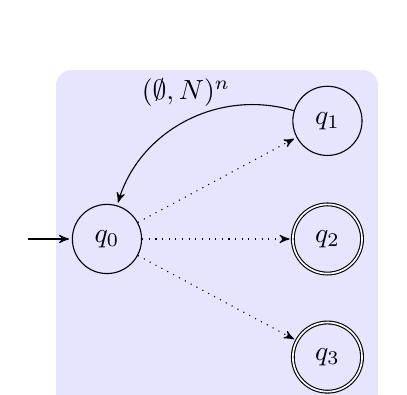
\begin{tikzpicture}[->,>=stealth',shorten >=1pt,auto,node distance=2.8cm,bend angle=45]
    \begin{scope}
      % Machine M
      \node[state]          (M init)                                    {$q_0$};
      \node[state]          (M exit 1)  [right of=M init,yshift= 1.5cm] {$q_1$};
      \node[state, double]  (M exit 2)  [right of=M init,yshift= 0.0cm] {$q_2$};
      \node[state, double]  (M exit 3)  [right of=M init,yshift=-1.5cm] {$q_3$};
      \path (M init)
      edge[dotted]          (M exit 1)
      edge[dotted]  (M exit 2)
      edge[dotted]  (M exit 3);
      \path (M init) ++(-1.0,0) edge (M init);
      \path (M exit 1) edge[bend right] node[anchor=south,yshift=0.2em] {$(\None, N)^n$} (M init);
    \end{scope}

    \begin{pgfonlayer}{background}
      \filldraw [line width=4mm,join=round,blue!10]
      (M   exit 1.north -| M   init.west) rectangle (M   exit 3.south -| M   exit 3.east);
    \end{pgfonlayer}
  \end{tikzpicture}

\end{document}

%%% Local Variables:
%%% TeX-master: t
%%% End:
  \caption{Example for $\While~M$ with $M:\TM_\Sigma^n(\Option(\Bool))$.  When the $M$ reaches the state $q_1$, the loop is continued, because $q_1$
    is in the partition $\None$ of $M$.  $q_2$ and $q_3$ are in the partition $\Some{\true}$ and $\Some{\false}$.  Therefore $\While~M$ terminates in
    its partition $\true$ or $\false$, when $M$ terminated in $q_2$ or $q_3$.}
  \label{fig:while-example}
\end{figure}

In Definition~\ref{def:While}, we have to assume that $F$ is inhabited.  However, the choice of $def:F$ is semantically irrelevant, because $\While~M$
only halts in states where $part_M(q)$ has a $\Some{.}$ value.

The correctness of $\MS{While}$ can be easily expressed using the following relation:

\begin{definition}[$\MS{WhileRel}$]
  \label{def:While_Rel}
  Let $R \subseteq \Tape_\Sigma^n \times \Option(F) \times \Tape_\Sigma^n$.  $\MS{WhileRel}~R \subseteq \Tape_\Sigma^n \times F \times \Tape_\Sigma^n$
  is defined inductively by the following two rules:
  \[
    \inferrule{R~t~(\None, t') \and \MS{WhileRel}~R~t'~(y, t'')}{\MS{WhileRel}~R~t~(y, t'')}
    \quad
    \inferrule{R~t~(\Some y, t')}{\MS{WhileRel}~R~t~(y, t')}
  \]
\end{definition}

We can also express this relation using the Kleene star:

\begin{lemma}[Alternative specification of $\While~M$]
  ~
  \[
    \MS{WhileRel}~R \equiv (R \at \None)^* \circ \Bigl( \bigcup_{y:F} \bigl( R \at {\Some y} \bigr) \att y \Bigr)
  \]
  (Where $\equiv$ means relational equivalence.)
\end{lemma}

Both definitions of $\MS{WhileRel}$ should make clear what $\While~M$ does: It repeats the execution of $M$ as long as it terminated in $\None$, and
after it terminated in $\Some y$, it terminates in the partition $y$.  This is visualised in Figure~\ref{fig:while-example}.  However, the inductive
definition is more practical when we prove correctness of concrete $\MS{While}$ machines, because we can just do induction on the inductive predicate.

\begin{lemma}[Correctness of $\MS{While}$]
  \label{lem:While_Realise}
  If $M \vDash R$, then $\While~M \vDash \MS{WhileRel}~M$.
\end{lemma}


We can not simply give a runtime relation in which $\While~M$ terminates, because we do not know the number of iterations in general.  However if we
know that $M$ realises $R$ and terminates in $T$, we can show $\While~M \downarrow T'$ for another runtime relation $T'$, if $T'$ ``decreases'' in
terms of $R$ and $t$:

\begin{lemma}[Runtime of $\While~M$]
  \label{lem:While_TerminatesIn}
  If $M \vDash R$, $M \downarrow T$.  We can show $\While~M \downarrow T'$ under the following assumption:
  \begin{multline*}
    \forall~t~i.~
    T'~t~i \rightarrow
    \exists~i_1.~
    \forall~t'.~ \\
    \bigl(
    \forall~y.~ R~t~(\Some y, t') \rightarrow i_1 \le i
    \bigl) ~\land~
    \bigl(
    R~t~(\None, t') \rightarrow
    \exists~i_2.~
    T'~t'~i_2 \land
    1 + i_1 + i_2 \le i
    \bigr)
  \end{multline*}
\end{lemma}

Note that we defined concrete correctness and termination relations for all combinators, but there is no known ``direct'' runtime Relation for
$\While$.  The best we could hope would be something like this relation:

\begin{definition}[Direct runtime relation for $\While$?]
  ~
  \[
    \inferrule{T~t~k \and R~t~(\Some y, t')}{WhileT~R~T~t~k}
    \quad
    \inferrule{T~t~k_1 \and R~t~(\None, t') \and WhileT~R~T~t'~k_2}{WhileT~R~T~t~(1+k_1+k_2)}
  \]
\end{definition}

However, when we try to prove $\While~M \downarrow WhileT~R~T$, we come to a goal where we have $R~t~(\Some y, t')$ and $R~t~(part_M(q''), t'')$, for
another final configuration $(q'',t'')$.  Thus, we can only prove $\While~M \downarrow WhileT~R~T$, if we assume that $R$ is functional:

\begin{lemma}[Direct runtime relation for $\While$]
  If $M \vDash R$, $M \downarrow T$, and $R$ is functional, then $\While~M \downarrow WhileT~R~T$.
\end{lemma}

However, our correctness relations are not functional in practice.  We encode preconditions in the relations, and if the precondition is not satisfied
for $t$, the value of $R~t~(y,t')$ simply is $\True$.  Therefore, we always use Lemma~\ref{lem:While_TerminatesIn} in practice.



\subsection{Proof of $\While$}
\label{sec:while-proofs}

The runtime and correctness proofs are similar to the proofs of $\Match$, as explained in Section~\ref{sec:match-proofs}.  However, the
configurations of $\Match$ are exactly the configurations of $M$, so the lifting function is the identity function.  The fundamental difference
between $\Match$ and $\While$ is that $\While$ can execute $M$ arbitrary often.  As a consequence, we also need complete induction over step-numbers,
in addition to the loop-splitting and loop-merging lemmas.  We present the key lemmas here and the most important parts of the proofs.

We simply write $\While$ instead of $\While~M$ in this section.  Since we have $\Conf_M = \Conf_\While$, we also only write $\Conf$.

The first lemma says that an execution of $\While$ consists of an execution of $M$ and a (possibly empty) continuation of $\While$:
\begin{lemma}[Splitting the execution of $\While$]
  \label{lem:While_split}
  Let $c_1, c_3 : \Conf$ and $k:\Nat$.  Then
  \begin{alignat*}{1}
    & \While(c_1) \terminates^k c_3 \rightarrow \\
    & \exists (k_1~k_2 : \Nat)~c_2. \\
    & \quad M(c_1) \terminates^{k_1} c_2 ~\land~ \\
    & \quad \While(c_2) \terminates^{k_2} c_3 ~\land~\\
    & \quad k_1 + k_2 \leq k.
  \end{alignat*}
\end{lemma}
\begin{proof}
  Follows with Lemma~\ref{lem:loop_split} and Lemma~\ref{lem:loop_lift}.
\end{proof}

We have two more splitting lemmas, for that case that $\While$ terminated immediately, and for that case that $\While$ continued the loop.
\begin{lemma}[Splitting, break case]
  \label{lem:While_split_term}
  Let $c_1 = (q, t)$, $c_2 : \Conf$, $k:\Nat$, and $y:F$.
  \begin{alignat*}{1}
    & \While(c_1) \terminates^k c_2 \rightarrow \\
    & haltConf_M~c_1 \rightarrow \\
    & part_M(q) = \Some y \rightarrow \\
    & c_2 = c_1.
  \end{alignat*}
\end{lemma}
\begin{proof}
  By Lemma \ref{lem:loop} (\ref{lem:loop_eq_0}), because $c_1$ is a halting state of $\While$.
\end{proof}
\begin{lemma}[Splitting, continue case]
  \label{lem:While_split_repeat}
  Let $c_1 = (q, t)$, $c_2 : \Conf$, $k:\Nat$.
  \begin{alignat*}{1}
    & \While(c_1) \terminates^k c_2 \rightarrow \\
    & haltConf_M~c_1 \rightarrow \\
    & part_M(q) = \None \rightarrow \\
    & \exists k'.~k = 1+k' ~\land~ \While(t) \terminates^{k'} c_2.
  \end{alignat*}
\end{lemma}
\begin{proof}
  $\While$ must have taken the ``nop''-transition from $c_1$ to $initConf~t$.
\end{proof}

We now can prove the correctness Lemma~\ref{lem:While_Realise} of $\While$.
\begin{proof}
  We assume $\While(t_1) \terminates^k c_3$ and have to show $WhileRel~t_1~(y, t_3)$.  We use complete induction on $k:\Nat$.  By
  Lemma~\ref{lem:While_split}, we have $M(t_1) \terminates^{k_1} c_2$ and\\ $\While(c_2) \terminates^{k_2} c_3$, for $k_1+k_2 \leq k$.  Case
  analysis.
  \begin{enumerate}
  \item $part_M(q_2) = \Some{y}$.  Then we know by Lemma~\ref{lem:While_split_term}, that $c_2=c_3$.  It remains to show $WhileRel~t_1~(y, t_2)$.  By
    applying the second constructor, it is enough to show $R~t_1~(\Some{y}, t_2)$.  This follows from the realisation of $M$.
  \item $part_M(q_2) = \None$.  By Lemma~\ref{lem:While_split_repeat}, we know that $\While(t_2) \terminates^{k'_2} c_3$ for $k_2 = 1 + k'_2$.  The
    inductive hypothesis gives $WhileRel~t_2~(part_\While~q_3, t_3)$.  The goal follows by applying the first constructor and the realisation of $M$.
  \end{enumerate}
\end{proof}


For the runtime proofs, we again have lemmas that ``merge'' steps together.

\begin{lemma}[Merging, break case]
  Let $k : \Nat$, $c_1, c_2 : \Conf$, and $y:F$.
  \begin{alignat*}{1}
    & M(c_1) \terminates^k c_2 \rightarrow \\
    & part_M(q_2) = \Some{y} \rightarrow \\
    & \While(c_1) \terminates^k c_2.
  \end{alignat*}
\end{lemma}
\begin{lemma}[Merging, continue case]
  Let $k_1, k_2 : \Nat$, $c_1, c_2, c_3 : \Conf$.
  \begin{alignat*}{1}
    & M(c_1) \terminates^{k_1} c_2 \rightarrow \\
    & part_M(q_2) = \None \rightarrow \\
    & \While(t_2) \terminates^{k_2} c_3 \rightarrow \\
    & \While(c_1) \terminates^{1+k_1+k_2} c_3.
  \end{alignat*}
\end{lemma}

The runtime Lemma~\ref{lem:While_TerminatesIn} follows similarly, by complete induction over $k:\Nat$.



\section{$\MS{Mirror}$}
\label{sec:mirror}

We can define a machine operator that ``mirrors'' a machine $M$.  Whenever $M$ makes a transition with a move to $L$, $\MS{Mirror}~M$ moves the head
to the right instead.  For example, we define a machine $MoveToSymbol$ below, that moves the head of the tape right, until it reads a certain symbol.
Using this operator, we get a machine ``for free'' that moves the head to the left instead.  Of course, the machine could be parametrised over the
direction.  However, in the correctness and termination proofs, we had to make case-distinctions over this direction parameter.  Essentially, this
repeats the proof.  However, we still have to copy or parametrise the correctness and runtime relations.

Using the proving techniques developed in the previous sections, verifying this $Mirror$ operator is very easy.

\begin{definition}[Mirror tape]
  \label{def:mirror_tape}
  Let $t : \Tape_\Sigma$.
  \begin{alignat*}{2}
    & \MS{mirror}~(\MS{niltape})         &&~:=~ \MS{niltape} \\
    & \MS{mirror}~(\MS{leftof}~l~ls)     &&~:=~ \MS{rightof}~l~ls \\
    & \MS{mirror}~(\MS{rightof}~l~ls)    &&~:=~ \MS{leftof}~l~ls \\
    & \MS{mirror}~(\MS{midtape}~ls~m~rs) &&~:=~ \MS{midtape}~rs~m~ls
  \end{alignat*}
\end{definition}
\begin{lemma}[Correctness of $\MS{mirror}$]
  \label{lem:mirror}
  Let $t,t':\Tape_\Sigma$.
  \begin{enumerate}
  \item \label{lem:mirror_tape_injective}
    $\MS{mirror}$ is injective, i.e.\ if $\MS{mirror}(t)=\MS{mirror}(t')$, then $t=t'$,
  \item \label{lem:mirror_tape_involution}
    $\MS{mirror}$ is an involution, i.e.\ $\MS{mirror}(\MS{mirror}(t))=t$,
  \item \label{lem:mirror_left}
    $\MS{left}(\MS{mirror}(t)) = \MS{right}(\MS{mirror}(t))$,
  \item \label{lem:mirror_right}
    $\MS{right}(\MS{mirror}(t)) = \MS{left}(\MS{mirror}(t))$,
  \item \label{lem:mirror_current}
    $\MS{current}(\MS{mirror}(t)) = \MS{current}(t)$.
  \end{enumerate}
\end{lemma}
\begin{proof}
  By case analysis over the tape(s).
\end{proof}


To define $\MS{Mirror}~M$, we assume an injective and involutive function $swap:\MS{Move} \to \MS{Move}$ that simply swaps $L$ and $R$.

\begin{definition}[$\MS{Mirror}~M$]
  \label{def:Mirror}
  Let $M:\TM_\Sigma^n(F)$.
  \[
    \delta(q, s) :=~
    \Let{(q', a) := \delta_M(q,s)}{\bigl(q', \map{(\lambda(w, m).~(w, swap(m)))}{a} \bigr)}
  \]
  (All other components are the same as $M$.)
\end{definition}

The correctness and termination proofs are similar to the proofs of $\MS{Match}$ and $\MS{While}$.  The ``lifting'' between configurations of $M$ and
$\MS{Mirror}$ is the injective and involutive function $mirrorConf : \Conf \to \Conf$ that simply mirrors the tapes.

\begin{definition}[Mirror configuration]
  \label{def:mirrorConf}
  Let $c : \Conf$.
  \[ mirrorConf(q,t) := (q, \map{mirror}{t}). \]
\end{definition}


\begin{lemma}[Mirroring steps]
  \label{lem:mirror_step}
  Let $c_1 : \Conf$.  Then
  \[ step_M~(mirrorConf~c_1) = mirrorConf~(step_{\MS{Mirror}}~c_1) \]
\end{lemma}

\begin{lemma}[Mirroring executions]
  \label{lem:mirror_loop}
  Let $c_1, c_2 : \Conf$.
  \begin{enumerate}
  \item \label{lem:mirror_split}
    $ \MS{Mirror} (c_1) \terminates^k c_2 \rightarrow M (mirrorConf~c_1) \terminates^k (mirrorConf~c_2) $
  \item \label{lem:mirror_merge}
    $ M (mirrorConf~c_1) \terminates^k (mirrorConf~c_2) \rightarrow \MS{Mirror} (c_1) \terminates^k c_2 $
  \end{enumerate}
\end{lemma}
\begin{proof}
  Claim~\ref{lem:mirror_split} follows with Lemma~\ref{lem:loop_unlift} and Lemma~\ref{lem:mirror_step}.  Claim~\ref{lem:mirror_merge} follows with
  Lemma~\ref{lem:loop_lift} and Lemma~\ref{lem:mirror_step}.
\end{proof}

\begin{lemma}[Correctness of $\MS{Mirror}$]
  Let $M \vDash R$.  Then $\MS{Mirror}~M \vDash MirrorRel~R$ with
  \[
    MirrorRel~R := \lambda t~(y, t').~ R~(mirror~t)~(y, mirror~t').
  \]
\end{lemma}
\begin{proof}
  Follows from Lemma~\ref{lem:mirror_loop}~(\ref{lem:mirror_split}).
\end{proof}
\begin{lemma}[Runtime of $\MS{Mirror}$]
  Let $M \vDash T$.  Then $\MS{Mirror}~M \downarrow MirrorT~T$ with
  \[
    MirrorT~T := \lambda t~k.~ T~(mirror~t)~k.
  \]
\end{lemma}
\begin{proof}
  Follows from Lemma~\ref{lem:mirror_loop}~(\ref{lem:mirror_merge}).
\end{proof}




\section{Partition Operators}
\label{sec:partition-op}

The operators of the above sections of this Chapter modified the behaviour of the machine.  However, we can also define simple operators that simply
modify the partitioning function $part : Q \to F$.  This is for example useful, if we want some (partitioned) machine to terminate in one particular
partition.

\begin{definition}[$\MS{ChangePartition}$]
  Let $M:\TM_\Sigma^n(F)$ and $g : F \to F'$.
  \[ \MS{ChangePartition}~M~g := (M, part_M \circ g). \]
\end{definition}

\begin{definition}[Fix partition]
  Let $M:\TM_\Sigma^n(F)$ and $y:F$.
  \[ \MS{Return~M~y} := \MS{ChangePartition}~M~(\lambda \_.~y). \]
\end{definition}

The correctness for these simple operators is obvious.  We do not even need lemmas for runtime, because the Definition~\ref{def:TerminatesIn} of
runtime is defined over bare machine without partitioning function.
\begin{lemma}[Correctness of $\MS{ChangePartition}$ and $\MS{Return}$]
  If $M \vDash R$, then
  \begin{alignat*}{1}
    \MS{ChangePartition}~M~g & \vDash \bigcup_{y:F} (R \at y) \att {g(y)} \\
    \MS{Return}~M~y          & \vDash \Bigl( \bigcup_{y':F} R \at y' \Bigr) \att y
  \end{alignat*}
\end{lemma}
\begin{proof}
  By definition.
\end{proof}


\section{Examples}
\label{sec:combining-examples}





%%% Local Variables:
%%% TeX-master: "thesis"
%%% End:

\chapter{Lifting Machines}
\label{chap:lifting}

We observe that whenever we want to combine machines, the numbers of tapes and alphabets of all involved machines have to match.

For example, assume that we have a one-tape machine that moves the head to the right.  If we need a two-tape machine that moves both tapes to the
right, we would like to use sequential composition and move one tape after the other tape to right.  But we would need two two-tape machines: one that
moves the first tape to the right and one that moves the second tape to the right.  There are multiple ways to solve this problem.  For example, we
could define a class of $n$-tape machines that move the $i$th tape to the right and leave all other tapes unchanged.  However, it is in general easier
to build and prove correctness of small machines that operate on a minimal amount of tapes.  Asperti and Ricciotti~\cite{asperti2015} define an
injecting operator that translates an one-tape machine into a $(1+n)$-tape machine.  We generalise this approach and implement an operator that takes
an $m$-tape machine and yields an $n$-tape machine, where $m \le n$.

The second part of this problem is how to combine machines with different alphabets.  For example, if we have a machine $\MS{Add}$ that sums
(encodings of) natural numbers, we could want to build a machine $\MS{Sum}$ that sums numbers in a list of numbers.  Consider an alphabet
$\Sigma_\Nat$ where we could encode natural numbers on, and an alphabet $\Sigma_{\List(\Nat)}$ to encode lists of natural numbers.  If the alphabet
$\Sigma_\Nat$ is included in $\Sigma_{\List(\Nat)}$, we would like to lift $\MS{Add}$ to the alphabet $\Sigma_{\List(\Nat)}$, to define $\MS{Sum}$.

Asperti and Ricciotti~\cite{asperti2015} avoid the latter problem.  They consider a fixed alphabet to encode all needed data on, to implement a
universal Turing machine.  However, this approach does not scale.  When the alphabet has to be changed, for example because we have to add a new data
type, they also must change the definitions of all involved ``smaller'' machines.  That is why we also introduce an operator that lifts a machine to a
bigger alphabet.


\section{Tape-Lift}
\label{sec:n-Lift}
\setCoqFilename{FormalComplexity.TM.Lifting.LiftTapes}%

The tape-lift takes a machine $M:\TM_\Sigma^m(F)$ and a duplicate-free vector\footnote{ Note that instead of duplicate free index vectors
  $I:\Fin_n^m$, we could also use injective functions $f: \Fin_m \to \Fin_n$.  However, we choose index-vectors, because they are easier to define in
  Coq.}  $I: \Fin_n^m$, and yields a machine $\LiftTapes{M}{I} : \TM_\Sigma^n(F)$.  The tape of $\LiftTapes{M}{I}$ with the index $i = I[j]$ (with
$i:\Fin_n$, $j:\Fin_m$), behaves exactly as the tape $j$ of $M$. All other tapes of $\LiftTapes{M}{I}$ that are not in $I$, do not change.


The transition function of $\LiftTapes{M}{I}$ gets the $n$ read symbols and selects the $m$ relevant symbols.  Then it applies the transition function
$\delta_M$ with the selected symbols and the current state $q$.  $\delta_M$ yields an $m$-vector $act:\Act^m$ and the continuation state $q'$.  It
fills ``nop''-actions into $act$, to get an action vector $act':\Act^n$.

\begin{definition}[Vector selecting][select]
  \label{def:select}
  Let $X:\Type$, $m,n:\Nat$, $I : \Fin_n^m$, and $V : X^n$.
  \[ select~I~V := \map{\bigl(\lambda (j:\Fin_m).~V[j] \bigr)}{I}. \]
\end{definition}
\begin{lemma}[Correctness of $select$][select_nth]
  By definition, for $k:\Fin_m$, we have
  \[
    (select~I~V)[k]=V\bigl[I[k]\bigr].
  \]
\end{lemma}

\begin{definition}[Vector filling][fill]
  Let $X:\Type$, $m,n:\Nat$,$I:\Fin_n^m$, $init:X^n$, and $V:X^m$:
  \begin{alignat*}{3}
    & fill~(\nil      )&& ~init~V &~:=~& init \\
    & fill~(i \cons I')&& ~init~V &~:=~& replace~(fill~I'~(\tl V))~i~(\hd V)
  \end{alignat*}
  Where $replace : X^n \to \Fin_n \to X \to X^n$ replaces the $i$th element of a vector.
\end{definition}
\begin{lemma}[Correctness of $fill$]
  If $I$ is duplicate-free, then
  \begin{enumerate}
  \coqitem[fill_correct_nth] \label{lem:fill_correct_nth}
    If $I[j]=i$, then $(fill~I~init~V)[i] = V[j]$.
  \coqitem[fill_not_index] \label{lem:fill_not_index}
    If $i \notin I$, then $(fill~I~init~V)[i] = init[i]$.
  \end{enumerate}
\end{lemma}
\begin{proof}
  By induction on $I : \Fin_n^m$.
\end{proof}

\begin{definition}[$\LiftTapes{M}{I}$][LiftTapes]
  \label{def:LiftTapes}
  Let $M:\TM_\Sigma^m(F)$ and $I : \Fin_n^m$.  We define $\LiftTapes{M}{I} : \TM_\Sigma^n(F)$.  All components are the same as in $M$, except:
  \begin{alignat*}{2}
    &\delta(q,s) &~:=~& \Let{(q', act) := \delta_M(q, select~I~sym)}{\\%
    &            &~  ~& (q', fill~I~(\None,N)^n~act)}
  \end{alignat*}
\end{definition}

\begin{lemma}[Correctness of $\LiftTapes{M}{I}$][LiftTapes_Realise]
  \label{lem:LiftTapes_Realise}
  Let $M : \TM_\Sigma^m(F)$ and $I : \Fin_n^m$ a duplicate-free index-vector.  If $M \Realise R$, then $\LiftTapes{M}{I} \Realise \LiftTapes{R}{I}$ with
  \[
    \LiftTapes{R}{I} := \lambda t~(y,t').~ R~(select~I~t)~(y, select~I~t') \land \forall i:\Fin_n.~i \notin I \rightarrow t'[i]=t[i].
  \]
\end{lemma}

\begin{lemma}[Runtime of $\LiftTapes{M}{I}$][LiftTapes_TerminatesIn]
  \label{lem:LiftTapes_TerminatesIn}
  Let $M : \TM_\Sigma^m(F)$ and $I$ duplicate-free index-vector. If $M \TerminatesIn T$, then $\LiftTapes{M}{R} \TerminatesIn \LiftTapes{T}{I}$ with
  $
    \LiftTapes{T}{I} := \lambda t~k.~ T~(select~I~t)~k.
  $
\end{lemma}

The proofs are similar to the former proofs, i.e.\ using Lemma~\ref{lem:loop_lift} and Lemma~\ref{lem:loop_unlift} with the following configuration
lifting function:
\[
  selectConf(q,t) := (q, select~I~t).
\]

However, for the second part of the correctness, i.e.\ tapes that are not in $I$ do not change, we need another lemma about $loop$:

\begin{lemma}[Mapping loops][loop_map]
  \label{lem:loop_map}
  Let $A:\Type$, $f:A \to A$, $h:A \to\ Bool$.  Let $B:\Type$ and $g : A \to B$.  If $g(f~a)=g(a)$ for all $a:A$, then
  \begin{alignat*}{1}
    & \forall (k:\Nat)~(a_1~a_2 : A). \\
    & \quad loop~f~h~k~a_1 = \Some{a_2} \rightarrow \\
    & \quad g(a_1) = g(a_2).
  \end{alignat*}
\end{lemma}
\begin{proof}
  By induction on $k:\Nat$.
\end{proof}

We apply this lemma in the proof of Lemma~\ref{lem:LiftTapes_Realise} with $g := \lambda ((q,t):\Conf).~t[i]$.



\section{Alphabet-Lift}
\label{sec:sigma-Lift}
\setCoqFilename{FormalComplexity.TM.Lifting.LiftAlphabet}%

Let $M : \TM_\Sigma^n(F)$ be a machine over the alphabet $\Sigma$, and $f : \Sigma \hookrightarrow \Tau$ a retraction on another alphabet $\Tau$.
Note that then $\Tau$ has at least as many symbols as $\Sigma$.  We need a default symbol $def:\Sigma$.  In contrast to the default partition we
needed in the definition of $\While$, the choice of $def$ is semantically relevant.  This means that $def$ should be a symbol that $M$ does not expect
to read.  The alphabet-lift $\LiftAlphabet{M}{(f,def)} : \TM_\Tau^n$ is a machine over the bigger alphabet $\Tau$.

The transition function of the lifted machine $\LiftAlphabet{M}{(f,def)}$ reads the symbols \\$s :
(\Option(\Tape_\Tau))^n$.  It tries to translate these symbols to $s':(\Option(\Tape_\Sigma))^n$ using the partial inversion function $f^{-1} : \Tau
\to \Option(\Sigma)$.  However, if the symbol $\tau:\Tau$ has no corresponding symbol in $\Sigma$, it must be translated to
$def$ instead.  The transition function $\delta_M$ of $M$ yields the successor state $q'$ and a vector of actions $act: (\Option(\Sigma) \times
\MS{Move})^n$, which is translated using $f:\Sigma\to\Tau$ to $act' : (\Option(\Tau) \times \MS{Move})^n$.

\begin{definition}[$\LiftAlphabet{M}{(f,def)}$][LiftAlphabet]
  \label{def:LiftAlphabet}
  Let $f : \Sigma \Tau$, $def:\Sigma$, and $M : \TM_\Sigma^n(F)$.  We define the machine %
  $\LiftAlphabet{M}{(f,def)} : \TM_\Tau^n(F)$ with the same components as $M$, except:
  \begin{alignat*}{2}
    &\delta(q,s)    &~:=~& \Let{(q', act) := \delta_M(q, \map{(mapOpt~surject)}{s})}{\\%
    &               &~  ~& (q', \map{(mapAct~f)}{act})} \\
    & surject(\tau) &~:=~&
    \begin{cases}
      \sigma & f^{-1}(\tau) = \Some{\sigma} \\
      def & f^{-1}(\tau) = \None
    \end{cases}
  \end{alignat*}
  with the canonical functions $mapOpt: \forall (X~Y:\Type).~ (X \to Y) \to \Option(X) \to \Option(Y)$ and
  $mapAct : \forall (\Sigma~\Tau:\Type).~(\Sigma\to\Tau) \to \Act_\Sigma \to \Act_\Tau$.  All other components are the same as $M$.
\end{definition}

\setCoqFilename{FormalComplexity.TM.TM}%
For the correctness and runtime lemmas, we also need the canonical function
\[
  \coqlink[mapTape]{mapTape}:\forall (\Tau~\Sigma:\Type).~(\Tau\to\Sigma)\to\Tape_\Tau\to\Tape_\Sigma
\]
that maps every symbol on a tape.  We write $\coqlink[mapTapes]{mapTapes}$ for the respective tape-vector function.
\setCoqFilename{FormalComplexity.TM.Lifting.LiftAlphabet}%

\begin{lemma}[Correctness of $\LiftAlphabet{M}{(f,def)}$][LiftAlphabet_Realise]
  \label{lem:LiftAlphabet_Realise}
  If $M \Realise R$, then $\LiftAlphabet{M}{(f,def)} \Realise \LiftAlphabet{R}{(f,def)}$ with
  \[
    \LiftAlphabet{R}{(f,def)} := \lambda t~(y, t').~R~(mapTapes~surject~t)~(y, mapTapes~surject~t').
  \]
\end{lemma}

\begin{lemma}[Runtime of $\LiftAlphabet{M}{(f,def)}$][LiftAlphabet_TerminatesIn]
  \label{lem:LiftAlphabet_TerminatesIn}
  If $M \TerminatesIn T$, then $\LiftAlphabet{M}{(f,def)} \TerminatesIn \LiftAlphabet{T}{(f,def)}$ with
  \[
    \LiftAlphabet{T}{(f,def)} := \lambda t~k.~T~(mapTapes~surject~t)~k.
  \]
\end{lemma}

The proofs are analogous to the former proofs.  The configuration lifting is
\[
  \coqlink[surjectConf]{surjectConf} (q,t) := (q, mapTapes~surject~t).
\]



%%% Local Variables:
%%% TeX-master: "thesis"
%%% End:
\chapter{Compound Machines}
\label{cha:compound}

In this chapter, we build complex machines, using the combinators developed in Chapter~\ref{chap:combining}, as well as the tapes-lift of
Chapter~\ref{chap:lifting}.  However, we do not use the alphabet lift in this chapter.  We also prove correctness and runtime of these machines.

The general approach, when we prove correctness of a machine $M$, i.e.\ if we want to show $M \vDash R$, is to first define a relation $R'$ that $M$
realises.  For that, we use the correctness lemmas of the combinators, lifts, and all concrete machines ``involved''.  The main part of the proof is
applying Lemma~\ref{lem:Realise_monotone} and showing $R' \subseteq R$.  Note that the first part of the proof, i.e.\ generating the relation $R'$
such that $M \vDash R'$, is mechanical.  Indeed, we can automatise this step in Coq, see more in Chapter~\ref{chap:implementation}.

When $M$ always terminates in constant time $k$, we show $M \vDash^k R$ instead.  Using the monotonicity Lemma~\ref{lem:RealiseIn_monotone}, we can
prove correctness and (constant) runtime at once.

For (non-constant) runtime, we use the dual approach.  However, we have an exception for $\While$, where we have to apply
Lemma~\ref{lem:While_TerminatesIn} directly instead of using the anti-monotonicity Lemma~\ref{lem:TerminatesIn_monotone}.

\section{$\Nop$}
\label{sec:Nop}

Using the alphabet-lift (Definition~\ref{def:LiftAlphabet}) and $\MS{Null}$ (Definition~\ref{def:Null}), it is easy to define an $n$-tape machine
$\Nop : \TM_\Sigma^n$ for every alphabet $\Sigma$ and number of tapes $n$:
\begin{definition}[$\Nop$]
  $Nop := \LiftTapes{\MS{Null}}{\nil}.$
\end{definition}
Note that because $\MS{Null}$ is a 0-tape machine, and $\Nop$ is supposed to be an $n$-tape machine, the index-vector must be the vector
$\nil : \Fin_n^0$.

\begin{lemma}[Correctness of $\Nop$]
  \label{lem:Nop_Sem}
  $\Nop \vDash^0 NopRel$ with $NopRel := \lambda t~t'.~t'=t$.
\end{lemma}
\begin{proof}
  By applying monotonicity of $\vDash^\cdot$ (Lemma~\ref{lem:RealiseIn_monotone}) and the correctness of $\MS{Null}$ (Lemma~\ref{lem:Null_Sem}), it
  remains to show that $\LiftTapes{NullRel}{\nil} \subseteq NopRel$.  To show the equality $t'=t$ we show $t'[i]=t[i]$ for all $i:\Fin_n$.  This
  follows with the equality part of the relation $\LiftTapes{NullRel}{\nil}$, because $i \notin \nil$.
\end{proof}

Note that the correctness relation of $\Nop$ can also be expressed using the identity relation $Id$:
\[
  \MS{NopRel} \equiv Id.
\]
However, we have the convention to define relations of concrete machine (classes) in $\lambda$-notation, i.e.\ not using relational operators.  Also
note that the tape $t'$ is per convention always on the left side of the equality.  This convention makes rewriting of tapes uniform; therefore,
rewriting of tapes can be automatised in Coq.

\section{$\MS{WriteString}$}
\label{sec:WriteString}

The machine $\MS{WriteString}~d~str$ writes a fixed string $str:\List(\Sigma)$ in the direction $d$.  It is defined by recursion over the string:
\begin{definition}[$\MS{WriteString}$]
  \begin{alignat*}{3}
    &\MS{WriteString}~d~&&(\nil)         &~:=~& \Nop \\
    &\MS{WriteString}~d~&&(s \cons str') &~:=~& \MS{WriteMove}~s~d \Seq \MS{WriteString}~d~str'.
  \end{alignat*}
\end{definition}

Note that this is the our only machine we define per recursion.  However, the way we proof correctness in constant time (depending on the length of
$str$) is still the same.

The relation that $\MS{WriteString}$ ``automatically'' realises in $3 \cdot \length{str}$ steps is the following:
\begin{lemma}
  $\MS{WriteString}~d~str \vDash^{3 \cdot \length{str}} R'~d~str$ with
  \begin{alignat*}{3}
    &\MS{R'}~d~&&(\nil        ) &~:=~& NopRel \\
    &\MS{R'}~d~&&(s \cons str') &~:=~& DoActRel(\Some{s}, d) \circ \MS{R'}~d~str'.
  \end{alignat*}
\end{lemma}
\begin{proof}
  By induction on $str:\List(\Sigma)$, using the monotonicity Lemma~\ref{lem:RealiseIn_monotone}, the correctness of $Nop$ (Lemma~\ref{lem:Nop_Sem}),
  the correctness of $\MS{WriteMove}$ (which is defined by $\MS{DoAct}$; Lemma~\ref{lem:DoAct_Sem}), and correctness of sequential composition for
  constant time (Lemma~\ref{lem:Seq_RealiseIn}).
\end{proof}
\todo{I don't have corollaries yet about seq, and if, and $\vDash^\cdot$.}

We define the actual relation of $\MS{WriteString}$ in terms of a recursive function on tapes:
\begin{lemma}[Correctness of $\MS{WriteString}$]
  \label{lem:WriteString_Sem}
  Let $d:\Move$ and $str:\List(\Sigma)$.
  \[ \MS{WriteString}~d~str \vDash^{4\cdot\length{str}} WriteStringRel~d~str \]
  with
  $WriteStringRel~d~str := \lambda t~t'.~t' = WriteStringFun~d~t~str'$ and
  \begin{alignat*}{3}
    &WriteStringFun~d~t~&&(\nil        ) &~:=~& t \\
    &WriteStringFun~d~t~&&(s \cons str') &~:=~& WriteStringFun~d~\bigl(doAct~t~(\Some{s}, d)\bigr)~str'
  \end{alignat*}
\end{lemma}
\begin{proof}
  We apply the monotonicity Lemma~\ref{lem:RealiseIn_monotone} and have to show\\
  $R'~d~str \subseteq WriteStringRel~d~str$.  We show this by induction on $str$.
\end{proof}

Note that we could as well use the $\MS{Mirror}$ operator instead of parametrising the machine $\MS{WritingString}$ over the direction.  However, in
this particular example, this approach seems to be easier.

\section{$\MS{MovePar}$}
\label{sec:MovePar}

The two-tape machine $\MS{MovePar}~d~d'$ combines two $\MS{Move}$ machines.  It first moves the $0$th\footnote{To avoid confusion with zero-based
  indices, we write the $0$th or $1$st tape, instead of the first or second tape.} tape in direction $d$ and after that the $1$st tape in
direction $d'$.
\begin{definition}[$\MS{MovePar}$]
  \label{def:MovePar}
  $\MS{MovePar}~d~d' := \LiftTapes{(\MS{Move}~d)}{\Vector{0}} \Seq \LiftTapes{(\MS{Move}~d')}{\Vector{1}}$.
\end{definition}
\begin{lemma}[Correctness of $\MS{MovePar}$]
  \label{lem:MovePar_Sem}
  $\MS{MovePar}~d~d' \vDash^3 MoveParRel~d~d'$ with
  \[ MoveParRel~d~d' := \lambda t~t'.~t'[0]=\MS{mv}~d~t[0] ~\land~ t'[1]=\MS{mv}~d'~t[1]. \]
\end{lemma}
\begin{proof}
  We have to show
  $$
    \LiftTapes{(\MS{DoActRel}(\None,d ))}{\Vector{0}} \circ
    \LiftTapes{(\MS{DoActRel}(\None,d'))}{\Vector{1}} \subseteq
    \MS{MovePairRel}~d~d'.
  $$
  We assume tapes $t, t', t''$ such that $(\LiftTapes{(\MS{DoActRel}(\None,d ))}{\Vector{0}})~t~t'$ and \\
  $(\LiftTapes{(\MS{DoActRel}(\None,d'))}{\Vector{1}})~t'~t''$, and have to show $t''[0]=\MS{mv}~d~t[0]$ and $t''[1]=\MS{mv}~d'~t[1]$.  By definition,
  we know $t'[0]=\MS{mv}~d~t[0]$ and $t'[1]=t[1]$ (because $1 \notin \Vector{0}$).  We also know $t''[1]=\MS{mv}~d'~t'[1]$ and $t''[0]=t'[0]$ (because
  $0 \notin \Vector{1}$).  The goal follows trivially.
\end{proof}
Note that this kind of proof is very mechanical: We only need to unfold the relations, and rewrite tapes.  Indeed, these steps are automatised in Coq.
Thus, we do not do more proofs of this kind on paper.

\section{$\MS{CopySymbols}$}
\label{sec:CopySymbols}

The machine $\MS{CopySymbols}~h : \TM_\Sigma^2$, where $h:\Sigma\to\Bool$, is a compound machine involving a $\While$-loop.  The machine reads the
symbol on tape $0$.  It reads the symbol on tape $0$ and writes it to tape $1$.  If the symbol fulfils $h$, then the machine halts.  Else it moves
both tapes right and continues the loop.  The machine also halts if there was no current symbol to read from tape $0$.

We first define the machine for the step.  Since we want to apply the $\While$ operator on the step machine, it must be partitioned over
$\Option(\Unit)$; $\Some\unit$ means break out of the loop and $\None$ means repeat the loop.
\begin{definition}[$\MS{CopySymbolsStep}$]
  \label{CopySymbols_Step}
  \begin{multline*}
    \MS{CopySymbolsStep}~f :=
    \Match(\LiftTapes{Read}{\Vector{0}}) \\
    \Biggl(
    \lambda s.
    \begin{cases}
      \Return{\bigl(\LiftTapes{(\MS{Write}~x)}{\Vector{1}}\bigr)}{\Some\unit} & s=\Some{x} ~\land~ f(x)=\true \\
      \Return{\bigl(\LiftTapes{(\MS{Write}~x)}{\Vector{1}} \Seq \MS{MovePar}~R~R\bigr)}{\None} & s=\Some{x} ~\land~ f(x)=\false \\
      \Return{\Nop}{\Some\unit} & s=\None
    \end{cases}
    \Biggr)
  \end{multline*}
\end{definition}

\begin{lemma}[Correctness of $\MS{CopySymbolsStep}$]
  \label{lem:CopySymbols_Step_Sem}
  ~
  \[
    \MS{CopySymbolsStep} \vDash^7 CopySymbolsStepRel
  \]
  with
  \begin{multline*}
    CopySymbolsStepRel := \lambda t~(y, t').~\\
    \begin{cases}
      t'[0] = t[0]           \land t'[1]=\MS{wr}~t[1]~\Some{x}         \land y=\Some\unit & \MS{current}~t[0]=\Some{x} \land       f(x) \\
      t'[0] = \MS{mv}~R~t[0] \land t'[1]=\MS{doAct}~t[1]~(\Some{x}, R) \land y=\None      & \MS{current}~t[0]=\Some{x} \land \lnot f(x) \\
      t' = t \land y=\Some\unit                                                           & \text{else}
    \end{cases}
  \end{multline*}
\end{lemma}
\todo{This looks \emph{ugly}!!!!!}
\begin{proof}
  Mechanical, with case-analysis over $t[0]$.
\end{proof}

Now, to define $\MS{CopySymbols}$, we simply apply the $\While$ operator to the step machine:
\begin{definition}[$\MS{CopySymbols}$]
  \label{def:CopySymbols}
  $\MS{CopySymbols}~f := \While(\MS{CopySymbolsStep}~f)$.
\end{definition}

The correctness of $\MS{CopySymbols}$ can be expressed using a recursive function on tapes:
\begin{lemma}[Correctness of $\MS{CopySymbols}$]
  \label{lem:CopySymbols_Realise}
  \
  $$\MS{CopySymbols}~f \vDash CopySymbolsRel~f$$
  with $CopySymbolsRel~f := \lambda t~t' = CopySymbolsFun~f~t$ and
  \begin{multline*}
    CopySymbolsFun~f~t :=\\
    \begin{cases}
      \Vector{t[0]; \MS{wr}~t[1]~(\Some{x})}                                  & \MS{current}(t[0])=\Some{x} \land f(x) \\
      CopySymbolsFun~f~\Vector{\MS{mv}~R~t[0]; \MS{doAct}~t[1]~(\Some{x}, R)} & \MS{current}(t[0])=\Some{x} \land \lnot f(x) \\
      t                                                                       & \MS{current}(t[0])=\None
    \end{cases}
  \end{multline*}
  Note that the function $CopySymbolsFun$ is not structural recursive.  It terminates because tapes have only finitely many symbols.
\end{lemma}
\begin{proof}
  To show: $WhileRel~CopySymbolsStepRel \subseteq CopySymbolsRel$.  By $\While$-induction (Lemma~\ref{lem:WhileInduction}).
\end{proof}

We observe that the runtime of $\MS{CopySymbols}$ only depends on the $0$th tape.  Therefore, we define a function
$CopySymbolsSteps : \Tape_\Sigma^n \to \Nat$ that overestimates the number of steps needed for the loop, depending on the $0$th tape.  Note that
$\While$ requires one additional step for each repeat of the loop.
\begin{lemma}[Runtime of $\MS{CopySymbols}$]
  $\MS{CopySymbols} \downarrow CopySymbolsT$ with \\
  $CopySymbolsT := \lambda t~k.~CopySymbolsSteps(t) \leq k$ and
  \begin{multline*}
    CopySymbolsSteps (t) := \\
    \begin{cases}
      8                                & \MS{current}(t)=\Some{x} \land f(x) \\
      8 + CopySymbolSteps(\MS{mv}~R~t) & \MS{current}(t)=\Some{x} \land \lnot f(x) \\
      8                                & \MS{current}(t)=\None
    \end{cases}
  \end{multline*}
\end{lemma}
\begin{proof}
  We use the termination Lemma~\ref{lem:While_TerminatesIn} of $\While$, with the correctness and (constant) runtime of $\MS{CopySymbolsStep}$
  (Lemma~\ref{lem:Realise_total} with Lemma~\ref{lem:CopySymbols_Realise}).\\
  Let $CopySymbolsSteps~t[0] \leq k$.  We have two cases.
  \begin{enumerate}
  \item We have $CopySymbolsStepRel~t~(\Some\unit, t')$.  Therefore, we know that either $\MS{current}(t[0])=\Some{x}$ with $f(x)=\true$, or
    $\MS{current}(t[0])=\None$.  In both cases, we have $CopySymbolsSteps(t[0]) = 8$.  Thus, we have
    $$ 7 \leq CopySymbolSteps(t[0]) = 8 \leq k. $$
  \item We have $CopySymbolsStepRel~t~(\None, t')$.  Therefore, we have $\MS{current}(t[0])=\Some{x}$ with $f(x)=\false$, and $t'[0]=\MS{mv}~R~t[0]$.
    Then, we have
    $$ 1+7+CopySymbolSteps(t'[0]) = CopySymbolSteps(t[0]) \leq k.$$
    \qed
  \end{enumerate}
\end{proof}
% Note that we see in the proof that we could replace the $8$s in the non-recursive parts of the runtime functions with $7$s.



%%% Local Variables:
%%% TeX-master: "thesis"
%%% End:
\chapter{Programming Turing Machines}
\label{chap:programming}

We can define machines using primitive operations like $\MS{DoAct}$, and can combine machines in an imperative programming style.  However, our
imperative ``language'' still has no notion of values or data cells.  We want to use each tape as a data cell to store one variable.  Therefore, we
have to define what it means that a tape contains a value.  When we ``program'' Turing machines, instead of using basic machines, we only use machines
that directly change the value of a tape.  We use the combinators introduced in Chapter~\ref{chap:combining} to simulate control flow of imperative
programming languages.  Using the definition of value-containing, we specify a ``callee-saving'' convention for function computation.  We present a
generic pattern how to program and verify Turing machines and show more complex case studies.


\section{Value-Containing}
\label{sec:value-containing}

We first want to define what it means that a tape $t$ \emph{contains} a value $x$, written as $t \simeq x$.  Tapes, as defined in \ref{def:tape}, are
essentially a list of symbols, so we have to linearise values to strings.

\begin{definition}[Encodable types]
  We say that a type $X$ is \emph{encodable} over $\Sigma$, if there is a function $encode : X \to \List(\Sigma)$.
\end{definition}

Morally, the encoding functions should be injective and there also should be a decoding function such that the encoding and decoding functions is a
retraction on $\List(\Sigma)$.  However, we do not need this strict definition.  We may encode a type $X$ on any alphabet $\Tau$, if $\Sigma$ is a
retraction on $\Tau$:
\begin{definition}[Map encodings]
  \label{def:Encode_map}
  Let $X$ be encodable over $\Sigma$ and $f : \Sigma \hookrightarrow \Tau$ be a retraction.  Then $X$ is also encodable over $\Tau$ with the following
  encoding function:
  \[ encode_\Tau(x) := encodeMap~encode_\Sigma~f~(x) := \map{f}{(encode_\Sigma(x))}. \]
\end{definition}
Note that mapping of encodings is compatible with composition of retractions.  This means that if we map the encoding twice, this is the same as
mapping the encoding with the composition of both retractions:
\begin{lemma}[Composition and encoding mapping]
  \label{lem:Encode_map_comp}
  Let $f : \Sigma \hookrightarrow \Tau$ and $g : \Tau \hookrightarrow \Delta$ be retractions and $X$ be encodable over $\Sigma$.  Then there is only
  one way how $X$ can be encoded over $\Delta$, i.e.:
  \[ encodeMap~(encodeMap~f~encode)~g~(x) = encodeMap~(f \circ g)~encode~x \]
\end{lemma}

For each type and type constructor, we have a disting alphabet.  We define basic encodings:
\begin{definition}[Basic encodings]
  \label{def:basic-encodings}
  \begin{enumerate}
  \item We encode $\Unit$ over the empty alphabet $\False$:
  \[ encode(\unit) := \nil
  \]
  \item The type $\Bool$ is encoded over itselve, i.e.\ $encode(b):=[b]$.
  \item Let $X$ be encodable over $\Sigma$.  Then $\Option(X)$ is encodable over
    \[ SigOpt~\Sigma ::= \MS{NONE} ~|~ \MS{SOME} ~|~ (x:\Sigma) \]
    With the retraction $RetrOpt : \Sigma \hookrightarrow SigOpt~\Sigma$ and
    \[
      encode(o) :=
      \begin{cases}
        [\MS{NONE}] & o=\None \\
        \MS{SOME} \cons encode(x) & x=\Some{x}
      \end{cases}
    \]
  \item Let $X$ be encodable over $\Sigma$ and $Y$ over $\Tau$.  Then $X+Y$ is encodable over
    \[ SigSum~\Sigma~\Tau ::= \MS{INL} ~|~ \MS{INR} ~|~ (x:\Sigma) ~|~ (y:\Tau) \] With the retraction
    $RetrOptX : \Sigma \hookrightarrow SigOpt~\Sigma~\Tau$ and $RetrOptY : \Tau \hookrightarrow SigOpt~\Sigma~\Tau$ and
    \[
      encode(s) :=
      \begin{cases}
        \MS{INL} \cons encode(x) & s=\inl x \\
        \MS{INR} \cons encode(y) & x=\inr y
      \end{cases}
    \]
  \item Let $X$ be encodable over $\Sigma$ and $Y$ over $\Tau$.  Then $X \times Y$ is encodable over
    \[ SigSum~\Sigma~\Tau ::= (x:\Sigma) ~|~ (y:\Tau) \] With the retraction
    $RetrSumX : \Sigma \hookrightarrow SigSum~\Sigma~\Tau$ and \\$RetrSumY : \Tau \hookrightarrow SigSum~\Sigma~\Tau$ and
    \[
      encode(s) :=
      \begin{cases}
        \MS{INL} \cons encode(x) & s=\inl x \\
        \MS{INR} \cons encode(y) & s=\inr y
      \end{cases}
    \]
  \item Let $X$ be encodable over $\Sigma$.  Then $\List(X)$ is encodable over
    \[ SigList~\Sigma ::= \MS{NIL} ~|~ \MS{CONS} ~|~ (x:\Sigma) \]
    With the retraction $RetrList : \Sigma \hookrightarrow SigList~\Sigma$ and
    \begin{alignat*}{3}
      &encode~&&(\nil      ) &~:=~& [\MS{NIL}] \\
      &encode~&&(l \cons ls) &~:=~& \MS{CONS} \cons encode(x) \app encode(ls)
    \end{alignat*}
  \end{enumerate}
\end{definition}

This are all encodings we need.  However, there is still a problem about ambiguity: Suppose $X$ is encodable over $\Sigma$.  Then the smallest
alphabet on which we can encode the type $X+X$ is $\Tau := SigSum~\Sigma~\Sigma$.  However, now there are two possibilities how to encode $X$ on
$\Tau$: using the retraction $RetrSigX$ and $RetrSigY$.  We must deal with this problem, when we program and prove Turing machines, by explicitely
giving the right retractions.

If $X$ is encodable over $\Sigma$, we encode values of $x$ on tapes with an extended alphabet $\Sigma^+$ that has an additional start and stop symbol.
\begin{definition}[$\Sigma^+$] Let $\Sigma$ be an alphabet.
  \[
    \Sigma^+ ::= \MS{START} ~|~ \MS{STOP} ~|~ \MS{UNKNOWN} ~|~ (s: \Sigma)
  \]
  Also, we define the retraction $RetrPlus : \Sigma \hookrightarrow \Sigma^+$.
\end{definition}
The $\MS{UNKNOWN}$ symbol is important later. We define what $t \simeq x$ means:
\begin{definition}[$t \simeq x$]
  \label{def:tape_contains}
  Let $X$ be encodable over $\Sigma$ and $t : \Tape_{\Sigma^+}$.
  \[
    t \simeq x := \exists~ls.~
    t = \MS{midtape}~ls~(\MS{START})~(encode(x) \app [\MS{STOP}])
  \]
  In case the encoding is not clear, we write $t \simeq_{f} x$ with $t:\Tape_{\Tau^+}$ and $x:X$, when $X$ is encodable on $\Sigma$ according to
  Definition~\ref{def:basic-encodings}, and we map this encoding to $\Tau$ using the retraction $f: \Sigma \hookrightarrow \Tau$.
\end{definition}

Note that in Definition~\ref{def:tape_contains}, we have to map the encoding of $x$ to the extended alphabet $\Sigma^+$.  If $t \simeq x$, the head of
$t$ stands on the start symbol.  To the right, there is the encoding terminated by the stop-symbol.  To the left of the head, there may be arbitrary
many ``rest'' symbols.

We found the convention useful, that there are no further symbols beyond the stop symbol.  In future work we also want to reason about space usage of
machines.  If a tape contains a value, the size of the tape (i.e.\ the number of symbols on it), only depends on the length of the encoding and the
number of rest symbols $ls$ to the left.  We have the convention to only add symbols to the left of a tape.  We also only write on tapes, if the head
of the tape is on the right-most symbol.

\section{Value-Manipulating Machines}
\label{sec:value-manipulate}


We defined what it means that a tape contains a value.  Now we want to define machines that manipulate values, e.g\ increase or increase a number.
Also, a very useful operation is to copy a value from one tape to another tape.


\todo{}







%%% Local Variables:
%%% TeX-master: "thesis"
%%% End:

\chapter{Simulating a Heap Machine}
\label{chap:heap}

In this chapter, we use all techniques, to implement a Turing machine that simulates an abstract heap machine.  First, we briefly define the semantics
of this abstract machine.  After that, we implement a Turing machine that simulates this machine and prove its correctness and polynomial runtime
overhead.  We show that this machine reduces the halting problem of the heap machine to the halting problem of multi-tape Turing machines.

\section{Heap Machine}
\label{sec:heap-def}

The abstract machine we present here is a variant of the heap machine in Kunze et~al.~\cite{KunzeEtAl:2018:Formal}.  Idem show that terms of the weak
call-by-value lambda-calculus can be refined to states of said abstract machine and formalise their results in Coq.
\todo{Should I include the compilation function $\gamma$ from lambda-terms to programs?}

Values of this machines are closures.  A closure is a program and a pointer to the environment of bindings.  This environment is implemented as a
linked list of closures.  Programs are lists of tokens, as defined below.
\begin{definition}[Programs, closures, and heaps]
  ~
  \begin{alignat*}{2}
    &Tok  &~::=~& \MS{VAR}(n:\Nat) ~|~ \MS{APP} ~|~ \MS{LAM} ~|~ \MS{RET} \\
    &Pro  &~:=~& \List(Pro) \\
    &Add  &~:=~& \Nat \\
    &Clos &~:=~& Add \times Pro \\
    &Entr &~:=~& \Option(Clos \times Add) \\
    &Heap &~:=~& \List(Entr)
  \end{alignat*}
\end{definition}

The states of the abstract machine are triples:
\[
  \Conf := \List(Clos) \times \List(Clos) \times Heap.
\]
The first list is the control stack and the second list is the value stack.  We define the small-step operational semantics of this machine as a
binary relation $\succ$ between states of the machine.
\begin{definition}[Semantics of the heap machine]
  {\small
    \begin{alignat*}{4}
      & \left((a, (\MS{LAM} \cons P)) \cons T, V, H\right)                      &~\succ~& \left((a, P') \cons_{tr} T, (a,Q) \cons V, H\right)
      \quad&& \text{if $\phi~P = \Some{(Q, P')}$} & \\
      & \left((a, (\MS{APP} \cons P)) \cons T, g \cons (b, Q) \cons V, H\right) &~\succ~& \left((c, Q) \cons (a,P) \cons_{tr} T, V, H'\right)
      \quad&& \text{if $put~H~\Some{(g,b)} = (c,H')$} \\
      & \left((a, (\MS{VAR}(n) \cons P)) \cons T, V, H\right)                   &~\succ~& \left((a, P) \cons_{tr} T, g \cons V, H\right)
      \quad&& \text{if $H[a,n]=\Some{g}$} &
    \end{alignat*}
  }
  with $put~H~c := (\length{H}, H \app [c]) $.\\
  We define $\phi~P :=~ \phi'~0~\nil~P$ with the auxiliary function $\phi' : \Nat \to Pro \to Pro \to \Option(Pro \times Pro)$, which is defined by
  recursion on $P:Pro$.
  \begin{alignat*}{4}
    &\phi'&~0~   &~Q&~(\MS{RET} \cons P) &&~:=~& \Some{(Q,P')} \\
    &\phi'&~(S~k)&~Q&~(\MS{RET} \cons P) &&~:=~& \phi'~k~(Q \app [\MS{RET}])~P \\
    &\phi'&~k    &~Q&~(\MS{LAM} \cons P) &&~:=~& \phi'~(S~k)~(Q \app [\MS{LAM}])~P \\
    &\phi'&~k    &~Q&~(t        \cons P) &&~:=~& \phi'~k~(Q \app [t])~P \\
    &\phi'&~k    &~Q&~              \nil &&~:=~& \None \\
  \end{alignat*}
  The heap lookup function $H[a,n] : \Option(Clos)$ is defined by recursion on $n$.
  \[
    H[a,n] :=
    \begin{cases}
      \Some{g}  & H[a]=\Some{\Some{(g,b)}} \land n=0 \\
      H[b, n-1] & H[a]=\Some{\Some{(g,b)}} \land n>0 \\
      \None     & \text{else}
    \end{cases}
  \]
  where $H[\cdot] : \Option(Entr)$ is the list lookup function. \\
  The tail-recursion optimised cons operation $\cons_{tr}$ is defined as follows:
  \begin{alignat*}{3}
    & (a, \nil) &~\cons_{tr}~& H &~:=~& H \\
    & (a, P   ) &~\cons_{tr}~& H &~:=~& (a, P) \cons H \qquad\text{if $P \neq \nil$}
  \end{alignat*}
\end{definition}

We write $\succ^k$ for the relational power (cf.\ Definition~\ref{def:pow}) and $\succ^*$ for the reflexive transitive closure of $\succ$ (cf.\
Definition~\ref{def:Kleene}).

The function $\phi$ matches $\MS{LAM}$ with $\MS{RET}$.  It splits the program into two parts, the first part is the ``body'' of a linearised lambda
expression and the second part the rest of the program, for example:%
{\small
  \[
    \phi[\MS{VAR}(0); \MS{LAM}; \MS{APP}; \MS{RET}; \MS{RET}; \MS{VAR}(1)] = \Some{([\MS{VAR}(0); \MS{LAM}; \MS{APP}; \MS{RET}], [\MS{VAR}(1)])}.
  \]
}%
The first $\MS{RET}$ matches to the $\MS{LAM}$ in the program above, so it is part of the first partition.  When the heap machine has a $\MS{LAM}$
token as first control token, it finds the rest of the program using $\phi$ and pushes the body on the control stack.

When the first control token is $\MS{App}$, the machine fetches two closures from the value stack.  The first closure, $g$, corresponds to the
parameter of the application.  The second closure, $(b,Q)$, corresponds to the called function.  The machine pushes $g$ on the heap.  After that it
continues executing $Q$, by adding a new closure $(c,Q)$ to the control stack, where $c$ is the updated head of the heap.

If the first control token is $\MS{VAR}(n)$, the machine looks up the $n$th entry in the environment on the heap at the address $a$, and pushes this
closure to the value stack.


\section{Implementation As Turing Machine}
\label{sec:heap-implementation}

We use the programming techniques from Chapter~\ref{chap:programming}.  For simplicity, we do not use the strict definition of functional computation.
The machines only save the input-values that the caller machines need again.  For example, we have a machine $\MS{Nth'}$ that saves the list, but not
the index.  The second change is that for functions with optional outputs, like $nth$, we do not extend the alphabet with $\Sigma_{\Option(X)}$.
Instead, we encode whether the output is $\Some{\cdot}$ or $\None$ with the partition $\Bool$.  In case that the output is $\None$, the machine
terminates in $\false$ and the output tape stays right.




\section{Reduction of the Halting Problem}
\label{sec:halting-problem}

% We can refine terms of closed lambda expressions to states of the abstract heap machine.  Hence, the halting problemm of lambda terms reduces to the
% halting problem of multi-tape Turing machines.



%%% Local Variables:
%%% mode: LaTeX
%%% TeX-master: "thesis"
%%% End:

\chapter{Conclusion}
\label{chap:conclusion}

% What we did and what others did
We have formalised multi-tape Turing machines in Coq.  We developed a framework for programming and proving correctness and runtime of multi-tape
Turing machines.  We have demonstrated the power of this framework by implementing a multi-tape Turing machine that simulates a two-stack abstract
machine.  This abstract machine is a variation from the heap machine in Kunze et~al.~\cite{KunzeEtAl:2018:Formal}.  The two variants of the heap
machine differ in that the programs in our version are linearised lists of tokens.  In~\cite{KunzeEtAl:2018:Formal}, the authors show that the states
of the heap machine can be \textit{refined} to terms of the programming language $L$, which is a subset of the call-by-value
$\lambda$-calculus\todo{Check!}.  It should be easy to formalise the reduction from the heap machine in~\cite{KunzeEtAl:2018:Formal} to our version of
the heap machine.  By that, we formalise the reduction from the halting problem of $L$ to the halting problem of multi-tape Turing machines.  This is,
however, outside the scope of this thesis.  Further possible future work include the formalisation of the reduction from multi-tape Turing machines to
single-tape Turing machines, and from single-tape Turing machines with arbitrary alphabet to single-tape Turing machines with a binary alphabet.  It
is an ongoing research project~\cite{ForsterLOLA}, to implement a Coq library of undecidability reductions, and this thesis provides one step towards
this goal.  The reduction from the Post correspondence problem (PCP) to the halting problem of single-tape Turing machines has already been formalised
in Coq in Heiter`s bachelor`s thesis~\cite{Heiter}.

\todo{The ``big picture'' from Yannick maybe would fit nice here}

% Differences and improvements to Asperti and other implementations
We build on Asperti and Ricciotti`s framework from~\cite{asperti2015} inside the theorem prover Matita and initially ported their definitions of tapes
and Turing machines to Coq.  We found their inductive definition of the tape in particular practical, because of its symmetric and final nature.  This
is in contrast to the implementation of tapes in~\cite{Xu:2013:MTM:2529315.2529331}, where tapes are split into two halves and the right half contains
the current symbol.  Because of the symmetric nature of tapes, it was extremely easy to define an operator $\MS{Mirror}$ that mirrors the transition
function.  The finite nature made it possible to define an always terminating machine that moves the head two the right (or using $\MS{Mirror}$ to the
left) end of the tape.  This is in contrast to~\cite{Ciaffaglione:2016:TTC:2956213.2956306}, where tapes are implemented as infinite streams of
symbols.  Our framework implements five major improvements on~\cite{asperti2015}.  (1) By introducing partitioned machines we make it unnecessary to
reason about concrete states of machines.  \cite{asperti2015} already note that reasoning about internal states is tedious and therefore do not
include the terminating state in their definition of realisation.  (2) We have introduced a notation of runtime.  Asperti and Ricciotti had two notion
of realisation, a strong and a weak one, where the former implies termination.  However, it made no commitments over the concrete number of steps
needed.  We use a variant of their weak notion of realisation and have introduced a new notion of runtime that relates the inputs to the number of
steps needed for the computation.  (3) By introducing an operator $\MS{Match}$ that generalises sequential composition and conditional, we simplified
the verification of both operators and also introduced a useful operator that was used throughout the thesis.  (4) We implemented general lifting
operators that make it possible to compose small machines (w.r.t.\ the alphabet and number of tapes) to fairly complex machines.  At this point,
composing compound machines is reasonable easy, but we (5) have introduced another layer of abstraction.  We have made it possible to directly
manipulate values of encodable types.  The on-paper design and implementation in Coq of the heap machine simulator was straight-forward.

% Duality Correctness and runtime
We noted that realisation and termination/runtime are dual in a sense.  The weak notion of realisation says that \textit{if} the machine terminates,
then the output is correct w.r.t.\ a correctness relation $R$.  On the other side, a machine terminates in a termination relation $T$ if all pairs of
input tapes $t$ and step numbers $k$, the machine terminates in $k$ with the input $t$.  Realisation is monotone (cf.\
Lemma~\ref{lem:Realise_monotone}) and termination is anti-monotone (cf.\ Lemma~\ref{lem:TerminatesIn_monotone}).  We found it remarkable that we use
an inductive correctness relation for $\MS{While}$ (cf.\ Lemma~\ref{lem:While_Realise} and a co-inductive termination relation (cf.\
Lemma~\ref{lem:While_TerminatesIn}).  We use induction show correctness and co-induction for termination of instances of $\While$.  Co-induction can
be however be avoided.  In fact, we introduced the co-inductive termination relation of $\While$ only for streamlines.

% Similarity of Realisation and weak Hoare triples
As already noted by~\cite{Ciaffaglione:2016:TTC:2956213.2956306}, the notion of realisation is similar to the classic Hoare logic widely used in
program verification.  For example, consider the classic Hoare proof rule for sequential composition:
\[
  \inferrule{\{A\}~P_1~\{B\} \and \{B\}~P_2~\{C\}}{\{A\}~P_1 \mathop; P_2~\{C\}}
\]
We encode preconditions and postconditions inside correctness relations.  This means that if the precondition is not true for the input tape $t$, then
$R~t~(y,t')$ is logically equivalent to $\True$.  We noted that sequential composition of machines amounts to relational composition of correctness
relations (cf.\ Lemma~\ref{lem:Seq_RealiseIn}).  However, we are not aware of a Hoare-style logical calculus for reasoning about termination in a
concrete number of steps and that is dual to classical Hoare logic, like in our duality between realisation and termination.

% Problems of the framework
The biggest problem of this framework is that encoding of types can be ambiguous.  For example, there are more than three ways how to encode natural
numbers on the alphabet of the heap machine simulator (cf.\ Section~\ref{sec:Lookup}).  We had to mentally keep track of in which encoding a value is
encoded on a tape, and to translate values from one encoding to another.

% Future work
When we defined the notion of value-containing (cf.\ Section~\ref{sec:value-containing}), we had \emph{future work} in mind where we formalise
space-usage of machines.  We can strengthen the correctness relations with assertions about the space-usage of each tape.  Asperti and Ricciotti`s
inductive definition of tapes is very helpful in this regard, because tapes never decrease the number of symbols.  This means that the total space
usage of a tape is just the number of symbols on the tape.  Our idea is that we parametrise the notion of value-containing over the length $l$ of the
``rest list'' on the left, and write $t \simeq_{l} x$.  Note that, by definition, there are no symbols beyond the stop symbol on the right side of the
tape, so the total size of the tape only depends of the length of the encoding and the length of the left rest.  For example, $\MS{MatchNat}$ does
change the amount of totally allocate memory, but decreases the length of the encoding and increases the length of the rest by one.  On the other
side, $\MS{ConstrS}$ ``consumes'' on rest symbol, i.e.\ decreases the length of the rest by one, and increases the length of the encoding by one.
Thus, if the rest is empty, $\MS{ConstrS}$ allocates one symbol.

Further future work could be to show that the runtime function of the simulator is polynomial w.r.t.\ the number of steps and the length of the
encoding of the initial heap machine state.


%%% Local Variables:
%%% TeX-master: "thesis"
%%% End:



\appendix

\addtocontents{toc}{\vspace{5mm}}
\chapter{Implementation in Coq}
\label{chap:implementation}

\lstset{style=coq}

% A full chapter for the implementation might not be worse it.  I think it is more important which libraries/plugins we use and how many lines of code
% do we need.  Does it really matter how we implement, e.g. tapes or Turing machines in Coq, because all definitions can be translated
% straight-forwardly to Coq.  The reader of the thesis can click on the theorems to read the source code, if he is interested.

We outline some pearls of the implementation of the framework of this thesis in the theorem prover Coq.  We do not assume additional axioms.  The
implementation compiles with the Coq versions 8.7 and 8.8.  We use proof scripts to derive proof terms in Coq, using Coq's standard tactical language
\textit{ltac}.

\section{Used Libraries}
\label{sec:coq-libraries}

Throughout the development, we make use of the \textit{typeclass} mechanism built into Coq.  Typeclasses are first-citizen objects in Coq, that may be
parametrised over types and other typeclasses.  Coq uses proof-search to infer instances of typeclasses.  For that, the user has to declare
definitions as typeclass instances.  We refer to Cast{\'e}ran and Sozeau~\cite{casteran2012gentle}, for a more thoughtful description of this feature.

\paragraph{Base Library and Finite Types}

We use a modified version of the library for the lecture \textit{Introduction to Computational Logic} by Prof.\ Smolka.  This library extends the
standard library of Coq with additional functions and automation for lists and decidable predicates.  On top of this library, we use the library of
finite types that was developed by Jan Menz in his bachelor's thesis \cite{JanMenz}.  The following listing outlines the definition of decidable
predicates and finite types:

\begin{lstlisting}
Definition dec (P:Prop) := {P} + {~ P}.
Definition eq_dec (X:Type) := forall x y, dec (x=y).
Structure eqType := EqType {
  eqtype :> Type;
  decide_eq : eq_dec eqtype
}.
Canonical Structure eqType_CS X (A: eq_dec X) := EqType X.
Class finTypeC (type: eqType) : Type := FinTypeC {
  enum : list type;
  enum_ok : forall x : type, count enum x = 1
}.
Structure finType : Type := FinType {
  type :> eqType;
  class : finTypeC type
}.
Canonical Structure finType_CS (X:Type) {p : eq_dec X} {class : finTypeC (EqType X)} : finType := FinType (EqType X).
\end{lstlisting}%

The coercions (\lstinline!:>!) make it possible to use finite types \lstinline{F:finType} as types, i.e.\ we can write \lstinline!x:F!.  The canonical
structures enable automatic inference of the structure, for example we have a function \lstinline!index : forall F:finType, F -> nat! and we can write
\lstinline!index true!.

\paragraph{Retraction Library}

We implemented a library for retractions.  We use a typeclass for the existence of retractions between two types.
\begin{lstlisting}
Section Retract.
  Variable X Y : Type.
  Definition retract (f : X -> Y) (g : Y -> option X) :=
    forall x y, g y = Some x <-> y = f x.
  Class Retract := {
    Retr_f : X -> Y;
    Retr_g : Y -> option X;
    Retr_retr : retract Retr_f Retr_g;
  }.
End Retract.
Arguments Retr_f { _ _ _ }.
Arguments Retr_g { _ _ _ }.
\end{lstlisting}
The \textit{Vernacular} command \lstinline!Arguments! makes $X$, $Y$, and the instance contextual implicit.  This means that
\lstinline!Retr_f : X -> Y!, where \lstinline!X! and \lstinline!Y! are inferred from the context.  We define instances for the retractions in
Section~\ref{sec:retracts}.

The retraction composition operator is not defined as an instance, to avoid diverging proof search during the typeclass inference, because it can be
applied arbitrary many times.  Although it is not declared as an instance of the typeclass of retractions, \lstinline!ComposeRetract! can be applied
manually.
\begin{lstlisting}
ComposeRetract : forall A B C : Type, Retract A B -> Retract B C -> Retract A C
\end{lstlisting}
We embed composition of retraction into retraction operators.  For example, instead of defining a retraction $RetrLft : X \hookrightarrow X+Y$, we
define (and declare as an instance) an operator on retractions:
\begin{lstlisting}
Retract_inl : forall A B C : Type, Retract A B -> Retract A (B + C)
\end{lstlisting}


\paragraph{Inhabited Types}
We also have a library for inhabited types.  Whenever we need a semantically irrelevant value, we can just write \lstinline!default! and Coq infers
the type and inserts a value with the following typeclass:
\begin{lstlisting}
Class inhabitedC (X : Type) :=
  {
    default : X;
  }.
\end{lstlisting}

\paragraph{Vectors and $\Fin_k$}

We use the type constructors \lstinline!Vector.t! and \lstinline!Fin.t! from Coq's standard library.  However, many basic lemmas and functions are
missing for this type.  We have a small library that adds the missing functions and lemmas.  It also provides some tactics, for example to make case
distinctions over \lstinline!Fin.t (S n)!.  We also introduce a notation for elements of $\Fin_k$.

\paragraph{smpl}

We use Sigurd~Schneider's smpl plugin \cite{SMPL}.  I lets the user add tactics to a tactic database and provides a tactic that applies the first
applicable tactic from the database.  We use this plugin for proof automation, more on that below.


\section{Value-containing}
\label{sec:coq-values}

The Coq implementation of the definition of multi-tape Turing machines is straight-forward.  Therefore, we omit code-listings here.  The interested
reader of the PDF version of this thesis might click on the definitions, to get to the Coq definitions.

We also use typeclasses to implement the notion of encodable types and value-containing.

\begin{lstlisting}
Section Codable.
  Variable (sig: Type).
  Variable (X: Type).
  Class codable := mk_codable {
    encode :> X -> list sig
  }.
End Codable.
Arguments encode {sig} {X} {_}.
Coercion encode : codable >-> Funclass.
\end{lstlisting}

The \lstinline!Coercion! vernacular makes is possible to write \lstinline!cX x!, when \lstinline!cX! is an instance that witnesses that \lstinline!x!
is encodable over \lstinline!X!.  This applies the concrete \lstinline!encode! function, given by \lstinline!cX!.  We prefer this notation over
\lstinline!encode x!, due to the fact that encodability is ambiguous, as noted in Section~\ref{sec:value-containing}.  We define the alphabets in
Definition~\ref{lem:retracts-basic} inductively, and also declare their proofs of finiteness.

We realise the type of the extended alphabet $\Sigma^+$ with $boundary + \Sigma$, where
\[ boundary ::= \MS{START} ~|~ \MS{STOP} ~|~ \MS{UNKNOWN} \]%
is defined as an inductive type.


\section{Automation}
\label{sec:coq-automation}

The Coq proof scripts make use of the builtin feature of \textit{existentials}.  An existential $?X$ is a type (that may contain variables referring
to more existentials) and the environment in which this existential should be typed.  Existentials are refined during unification (e.g.\ using the
\lstinline!apply! tactic) in the proof script.  Before the proof script can be finished and saved with the \lstinline!Qed! command, all existential
variables must be bound to values.

The tactic \lstinline!TMSimp! destructs conjunctive assumptions in all hypothesises (i.e.\ logical conjunctions and logical existentials).  It also
names introduced tapes to \lstinline!tmid!, \lstinline!tmid0! etc.  Furthermore, it instantiates and rewrites with hypothesis of the form
$H: \forall j.~ j \notin I \rightarrow tmid0[j] = tmid[j]$, that come from the correctness Lemma~\ref{lem:LiftTapes_Realise} of the tapes-lift
operator.

The tactic \lstinline!modpon H! instantiates assumptions of the form $H: \forall x~\cdots.~P \rightarrow \cdots \rightarrow Q$.  For each premise that
the tactic could not solve automatically, it creates a new subgoal with existentials for the quantified variables.

The tactic \lstinline!repeat TM_Correct! instantiates the existential relation $?R'$ and proves $M \Realise ?R'$.  For that, it applies all
correctness lemmas of the combinators, lifts, value-constructors and deconstructors, and some other auxiliary machines.  It does not apply correctness
lemmas that are parametrised over an encoding function, e.g.\ the correctness Lemma~\ref{lem:CopyValue_Realise}, because the choice of the encoding
functions is semantically relevant.  The user can declare more correctness and runtime lemmas to be used by \lstinline!TM_Correct!.  We use the Coq
plugin \textit{smpl} (see~\cite{SMPL}).  For example, the following code declares the correctness and runtime lemmas of \lstinline!LiftTapes!:

\begin{lstlisting}
Ltac smpl_TM_LiftN :=
  lazymatch goal with
  | [ |- LiftTapes _ _ $\Realise$ _] =>
    apply LiftTapes_Realise; [ smpl_dupfree | ]
  | [ |- LiftTapes _ _ $\Realise$c(_) _] =>
    apply LiftTapes_RealiseIn; [ smpl_dupfree | ]
  | [ |- projT1 (LiftTapes _ _) $\TerminatesIn$ _] =>
    apply LiftTapes_Terminates; [ smpl_dupfree | ]
  end.
Smpl Add smpl_TM_LiftN : TM_Correct.
\end{lstlisting}
The tactic \lstinline!smpl_dupfree! automatically proves that a vector is duplicate-free.


\section{Example Correctness Proof in Coq}
\label{sec:coq-correctness}

We use the general approach how to prove correctness (or runtime) of a Turing machine, as described in Chapter~\ref{chap:compound}: We show
$M \Realise R'$ for some relation $R'$ and it remains to show $R' \subseteq R$.  The first step is done using the tactic
\lstinline!rrepeat TM_Correctr!  For example, consider the following goal (we use the user-defined Coq notation \lstinline!$\Realise$c(9)! to mean
$\RealiseIn{9}$).
\begin{lstlisting}
============================
Add_Step $\Realise$c(9) Add_Step_Rel
\end{lstlisting}
The outline of the proof script is:
\begin{lstlisting}
Proof.
  eapply RealiseIn_monotone.
  { unfold Add_Step. repeat TM_Correct. }
  { cbn. reflexivity. }
  { (* ... *) }
Qed.
\end{lstlisting}

The tactic \lstinline!eapply RealiseIn_monoton! applies Lemma~\ref{lem:Realise_monotone}, and creates \textit{existential} variables $?R'$ and $?k'$.
The tactic generates three goals:
\begin{lstlisting}
3 focused subgoals
(shelved: 2)
  
============================
Add_Step $\Realise$c(?k') ?R'

subgoal 2 is:
 ?k' <= 9
subgoal 3 is:
 ?R' <<=2 Add_Step_Rel
\end{lstlisting}

After focusing the first subgoal, we unfold the definition of \lstinline!Add_Step!:
\begin{lstlisting}
============================
If (LiftTapes MatchNat [|Fin1|])
   (Return (LiftTapes Constr_S [|Fin0|]) None)
   (Return Nop (Some tt)) $\Realise$(?k') ?R'
\end{lstlisting}

The tactic \lstinline!repeat TM_Correct! automatically applies the correctness lemmas of the conditional, tape-lifting, etc.  It instantiates
\lstinline!?R'! to the following relation:
\begin{lstlisting}
?R' := (LiftTapes_Rel [|Fin1|] MatchNat_Rel|_true $\circ$
        ($\bigcup_{f:\Unit}$ LiftTapes_Rel [|Fin0|] S_Rel|_f)||_None)
       $\cup$
       (LiftTapes_Rel [|Fin1|] MatchNat_Rel|_false $\circ$
        ($\bigcup_{f:\Unit}$ Nop_Rel|_f)||_(Some tt))
\end{lstlisting}
It also instantiates
\begin{lstlisting}
?k' := 1 + MatchNat_steps + Nat.max Constr_S_steps 0
\end{lstlisting}
where \lstinline!MatchNat_steps! is the constant number of steps required for $\MS{MatchNat}$ (i.e.\ $5$) and \lstinline!Constr_S_steps! is $3$.  By
simplification, the second goal reduces to \lstinline!9<=9!, which is solved by reflexivity of $\leq$.

The main part of the proof is the third goal.  We prove it with the following proof script:
\begin{lstlisting}
{
  intros tin (yout, tout) H. cbn. intros a b HEncA HEncB.
  cbn in *. destruct H; TMSimp.
  - modpon H. destruct b; auto.
  - modpon H. destruct b; auto.
}
\end{lstlisting}

After the introduction of the variables and hypothesises $tin[0] \simeq a$, $tin[1] \simeq b$, and \lstinline!H: R' tin (yout, tout)!, we make a
case-distinction over $H$ (note that the head-operator in the definition of $R'$ is $\cup$, so $H$ reduces to a disjunction).  This gives two
sub-goals.  In both subgoals, we use the automation tactic \lstinline!TMSimp!.

The first subgoal is:
\begin{lstlisting}
tin, tout, tmid : tapes (boundary + sigNat) 2
H : forall n : nat, tin[@Fin1] $\simeq$ n -> match n with
                               | 0 => False
                               | S n' => tmid[@Fin1] $\simeq$ n'
                               end
H0 : forall n : nat, tin[@Fin0] $\simeq$ n -> tout[@Fin0] $\simeq$ S n
a, b : nat
HEncA : tin[@Fin0] $\simeq$ a
HEncB : tin[@Fin1] $\simeq$ b
H0_0 : tmid[@Fin0] = tin[@Fin0]
H1_0 : tout[@Fin1] = tmid[@Fin1]
============================
match b with
| 0 => False
| S b' => tout[@Fin0] $\simeq$ S a /\ tmid[@Fin1] $\simeq$ b'
end
\end{lstlisting}

In this case, we know that $a$ must be equal to $S~a'$ for some $a'$.  The assumption $H$ is automatically instantiated with $n$ and the proof
$HEncA$.  We finish the goal by case-distinction over $a$.  The second goal is analogous.


Even for complex machines, the correctness proofs in Coq follow this pattern.  It is important to note that the structure of the proof always follows
the structure of the machine.  Runtime proofs are analogous.


\section{Lines of Code}
\label{sec:coq-lines}

In Table~\ref{tab:coq-lines}, we summarise the numbers of Coq code.  We used the tool \texttt{coqwc} to count the lines.%
\todo{This table is \textit{not} complete!}
% XXX: This table excludes:
% - TMTac, ProgrammingTools
\begin{table}[h]
  \centering
  \begin{tabular}{p{7cm}|r|r}
    Module                                    & Spec & Proof\\ \hline
    Libraries (incl. our code)                &  153 & 2638 \\
    Preliminary (incl. $\Loop$ and relations) &  228 &  197 \\
    Definition of Turing machines             &  448 &  180 \\
    Basic Machines                            &  122 &   34 \\
    Combinators                               &  422 &  383 \\
    Lifting                                   &  361 &  193 \\
    Compound Machines                         &  378 &  278 \\
    Value containing                          &  424 &  119 \\
    Copying and writing values                &  411 &  288 \\
    Alphabet-Lift with values                 &  134 &  269 \\
    Deconstructors and constructors           &  492 &  492 \\
    $\MS{MapSum}$                             &   47 &  298 \\
    Addition and Multiplication machines      &  181 &  298 \\
    List functions machines                   &  329 &  456 \\
    Heap Machine Simulator                    &  989 & 1057 \\ \hline\hline
    Total                                     & 7119 & 7180 \\
  \end{tabular}
  \caption{Lines of specification and proof code for the ``modules'' (with several source files)}
  \label{tab:coq-lines}
\end{table}



%%% Local Variables:
%%% TeX-master: "thesis"
%%% End:



\renewcommand{\emph}{\textit}

\bibliographystyle{plainnat}
\bibliography{mybibliography}

\end{document}

%%% Local Variables:
%%% mode: latex
%%% TeX-master: t
%%% End:
